\chapter{Identification of jets from bottom quarks}
Accurately identifying jets from bottom quarks is a crucial part of physics program involving top quarks, which decays before hadronization to b quarks and the W boson, and the Higgs boson, which decays primarily to b quarks. This amounts to measuring the quantum numbers of the partons that give rise to individual jets.

The relatively large lifetime, the hadronization properties of the bottom quark and the possible semileptonic decays of b~hadrons allow us to experimentally identify the jets that arise from bottom and charm quarks through the technique of b tagging, or more generally flavour tagging. A b quark has a relatively long lifetime of $10^{-12}$ seconds and a large Lorentz boost factor, resulting in hadronization at a decay vertex that is displaced by several millimetres with respect to the primary interaction point.

The idea of b tagging is to use a combination of discriminating variables to distinguish between jets from bottom, charm and light quarks on a statistical basis by assigning a discriminator value for jets that is on average higher for jets arising from bottom quarks than for the ones arising from light quarks. Jets that pass a certain pre-determined threshold of the discriminator value are taken to be tagged as a certain flavour. This technique based on the presence of a secondary vertex was first used at Tevatron in the analyses that led to the discovery of the top quark~\cite{Abe:1994st,Abe:1995hr}.

In this chapter, we will give an overview of b tagging at CMS, with a specific focus on the development and re-optimisation of the Combined Multivariate~(cMVAv2) b~tagging algorithm for Run II. We start with an overview of the discriminating variables important for b~tagging, followed by a description of the existing b~tagging algorithms at CMS. We then introduce the cMVAv2 algorithm and describe the optimisation and performance of the retrained version in Run II. We conclude with an outlook on flavour tagging. 

\section{Discriminating variables}
The most important discriminating variables for flavour tagging are the kinematic properties of jets and the associated leptons, as well as the existence and properties of tracks from charged particles and vertices associated to either the primary hard interaction in the proton-proton collision or the secondary vertices from the decay of b or c~hadrons. The secondary vertex of b~hadron decay, which is displaced with respect to the primary vertex due to the long life time of b~hadrons, is an especially salient feature of b~hadron decays that the b~tagging algorithms seek to exploit through accurate track and vertex reconstruction. Therefore, the selection of good tracks and the reconstruction of secondary vertices is necessary for efficient b~tagging.

\subsection{Track selection}
The tracks reconstructed by the inner tracking detector and associated to jets are used for b~tagging only in case they are of sufficient quality, i.e. they pass the track selection. This means they must have a transverse momentum of at least~1~GeV, a normalized~$\chi^2$~quality parameter for the fit to hits below~5 and at least~8 hits in the tracker with at least 2 in the inner pixel detector. Furthermore, the impact parameter~(IP), shown on \cref{fig:btag_ip}, is defined as the distance of closest approach between the primary vertex and the track trajectory is required to be less than~0.2~(17)~cm in the transverse~(longitudinal) direction to ensure that the tracks are sufficiently close to the primary vertex and thus reduce the contribution from pileup. The distance of closest approach between the jet and the track must be smaller than~0.07~cm and the decay length, defined as the distance between the primary vertex and the point of closest approach between the track and the jet must be less than~5~cm. Jets at $p_T = 100~\mathrm{GeV}$~are estimated to have around 7 associated tracks, with the multiplicity rising significantly at higher momenta. \cite{CMS-PAS-BTV-15-001}.

\begin{figure}
\begin{centering}
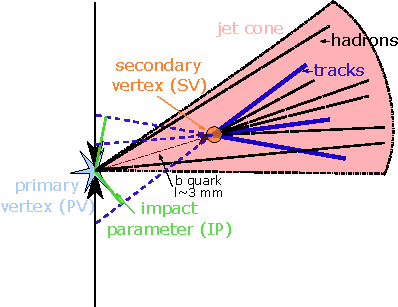
\includegraphics[width=0.4\textwidth]{figures/btv/ip.pdf}
\caption[Illustration of b~quark decay]{An illustration of the decay of a b~quark, along with the definition of the secondary vertex and the impact parameter.}
\label{fig:btag_ip}
\end{centering}
\end{figure}


\subsection{Vertex reconstruction}
Tracks passing the pileup-suppressing selection selection are used for vertex reconstruction in the adaptive vertex reconstruction~(AVR) algorithm~\cite{Waltenberger:2008zz}. Vertices reconstructed by AVR must pass further selection criteria designed to suppress vertices that are unlikely to originate from b~hadron decay. These selection criteria require a vertex to have a sufficient number unique tracks, a high-significance flight distance, a mass of less than~6.5~GeV and incompatible with the~$K_S^0$~hadron. Upon fulfilling these criteria, a jet is assigned to contain an AVR vertex~\cite{CMS-PAS-BTV-15-001}.

An alternative to AVR, where tracks are required to be associated to jets and therefore vertex reconstruction is seeded by jets, is the inclusive vertex finder~(IVF) algorithm~\cite{Khachatryan:2011wq}. As the name implies, the IVF algorithm starts with the set of all tracks in the event that pass somewhat looser selection criteria than used for AVR. Vertices are found by fitting all tracks simultaneously using an adaptive fitting algorithm looking for clusters of tracks. A further arbitration step assigns tracks to either the primary or secondary vertex based on compatibility and pixel hits, or removes secondary vertices of low quality. The IVF algorithm reconstructs about~10~\%~(15~\%)~more often the vertices from bottom~(charm) hadrons, but also increases the fraction of vertices reconstructed for light jets by about~8~\%. The overlap between the two algorithms is about~60\%, meaning that both vertex fitters provide some independent information on the event~\cite{CMS-PAS-BTV-15-001}.

\section{Multivariate b~taggers}
Using machine learning, signals from various regions of the detector can be combined effectively to develop a discriminator between b jets and light jets. Such techniques are especially suited to exploit sources of information that are partially correlated, such as the AVR and IVF vertices. The cMVAv2 b~tagging algorithm combines the output of different low and high level b~tagging algorithms, developed independently and using partially correlated variables, into a single high level discriminator. Before we can describe the cMVAv2 in detail, we must therefore discuss the different b~tagging algorithms used at CMS.

\subsubsection{Jet probability taggers}
The Jet Probability (JP) tagger was developed during Run I and is a simple multivariate likelihood discriminator based on track properties. In JP, the likelihood for a jet to originate from the primary vertex, as opposed to a secondary vertex, is computed by multiplying the per-track likelihoods, based on the track impact parameter and detector resolution. In a version of the JP tagger, the 4 tracks that have the highest IP significance~($\mathrm{IP} / \sigma_{\mathrm{IP}}$) are given a higher weight such that the new tagger, denoted Jet B-Probability (JBP) is more efficient in discriminating against b jets~\cite{Chatrchyan:2012jua}. The discriminator distributions for the JP and JBP b~taggers are shown on~\cref{fig:btag_jbp}.

\begin{figure}
\begin{centering}
\subfloat[The JP b~tagger]{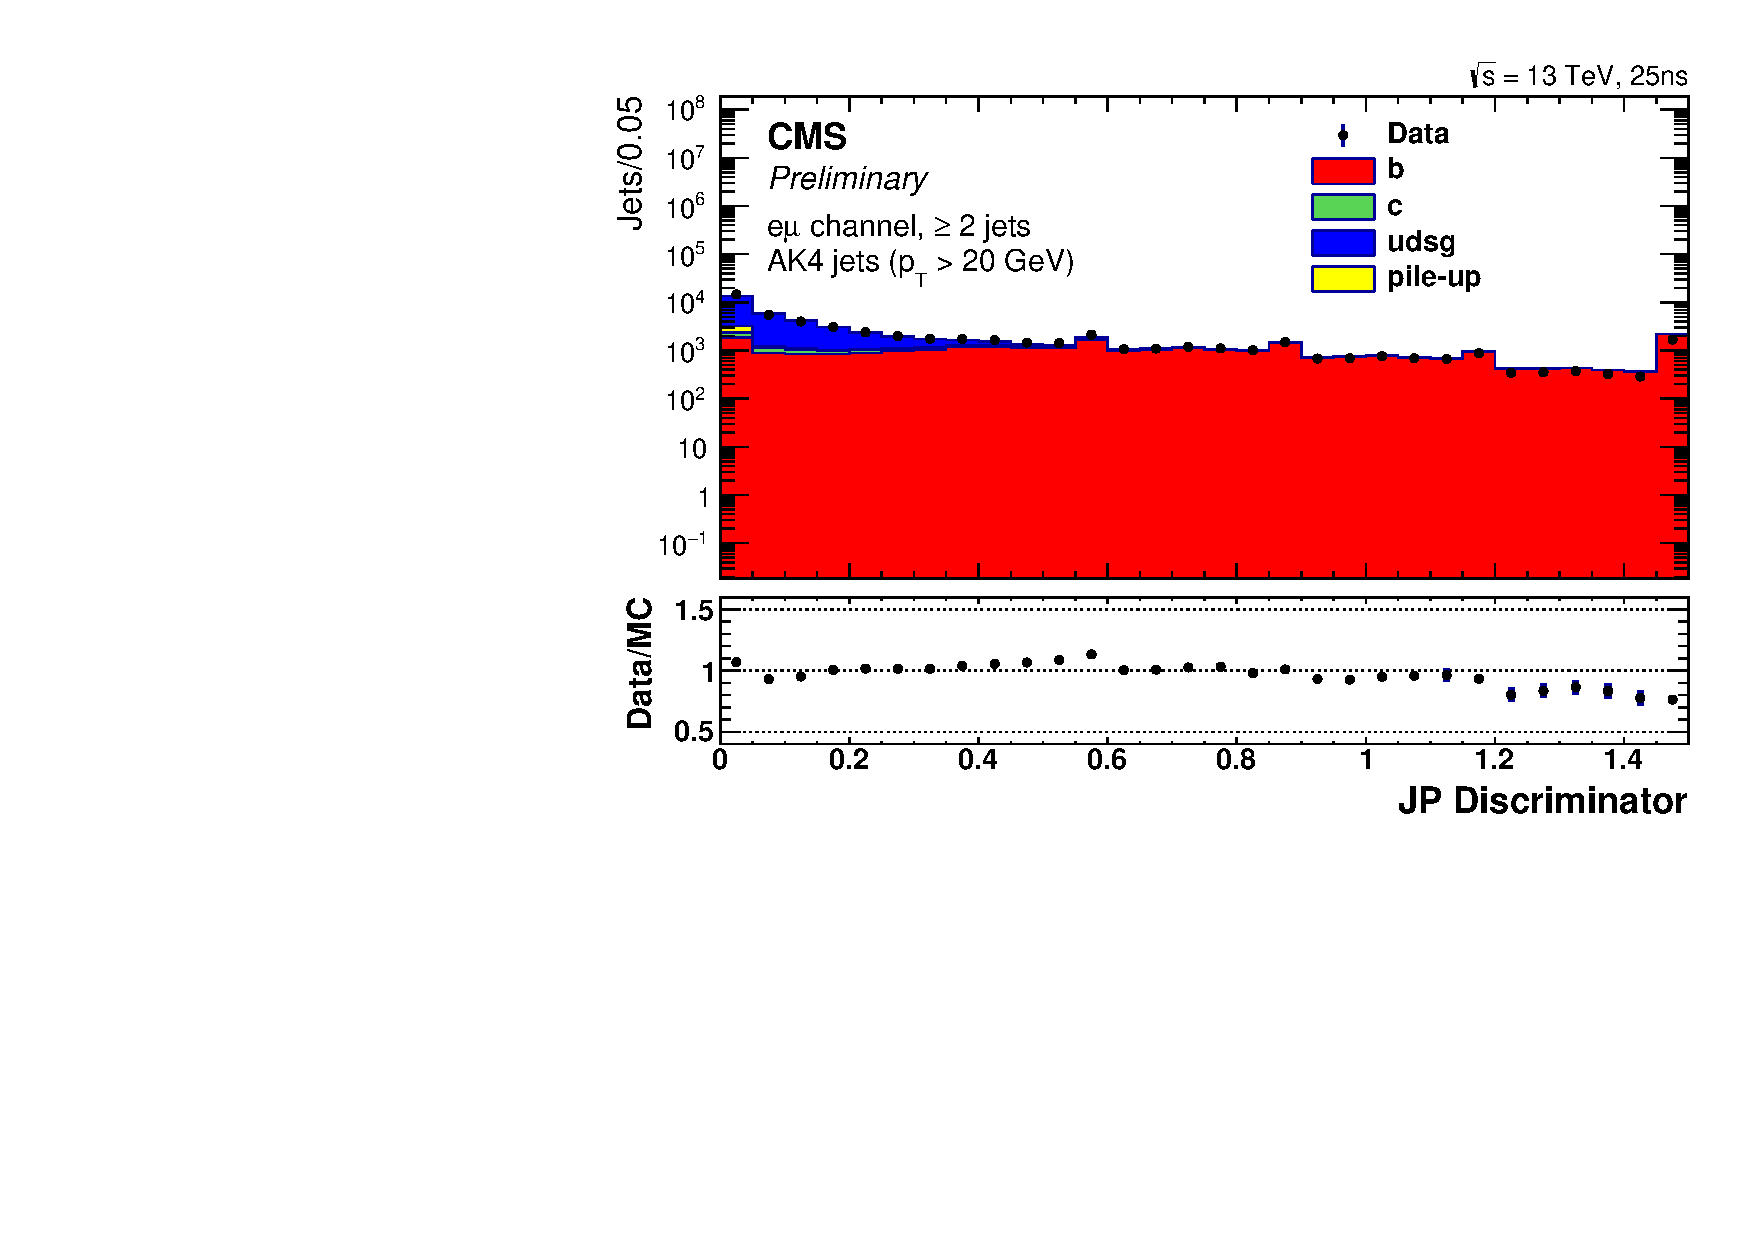
\includegraphics[width=0.5\textwidth]{figures/btv/jp.pdf}}
\subfloat[The JBP b~tagger]{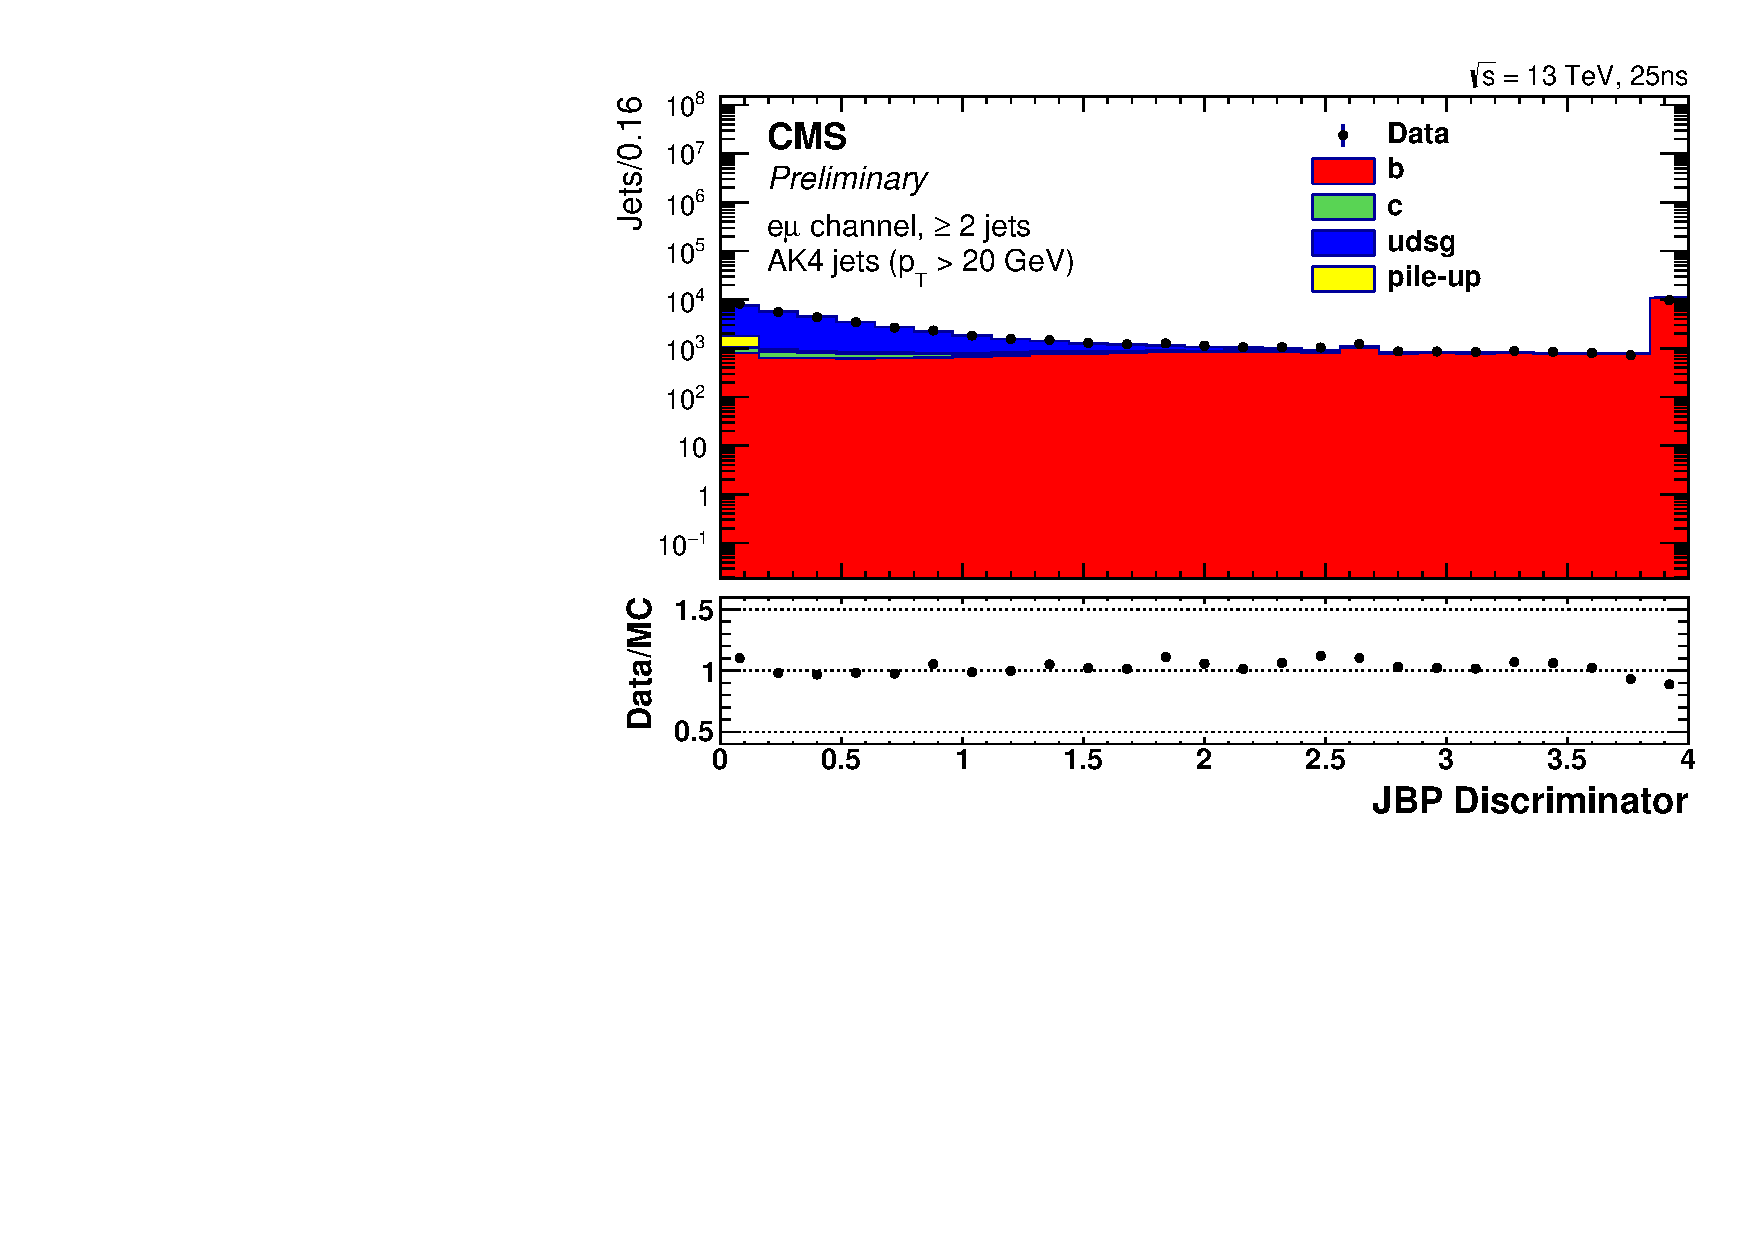
\includegraphics[width=0.5\textwidth]{figures/btv/jbp.pdf}} \\
\caption[The jet probability b discriminator distributions]{The jet probability b taggers in dileptonic ($\mathrm{e\mu}$) \ttbar+jets events. Figures from~\cite{CMS-PAS-BTV-15-001}.}
\label{fig:btag_jbp}
\end{centering}
\end{figure}

\subsubsection{Soft lepton taggers}
The semileptonic decays of the b~hadron to muons through~$\mathrm{b} \rightarrow \mathrm{\mu}^- \bar{\nu}_{\mathrm{\mu}} s$, which happens with a branching fraction of about~$20\%$, makes it possible to use the presence of a reconstructed muon in a jet for b~tagging. The Soft Muon (SM) algorithm in CMS relies on the presence of a muon in the jet constituents, but not on the presence of a secondary vertex. Similarly, the decay of a b~hadron to an electron is exploited through the Soft Electron (SE) tagger~\cite{CMS-PAS-BTV-15-001}. The discriminator distributions are shown on~\cref{fig:btag_softlep}.

\begin{figure}
\begin{centering}
\subfloat[The soft electron b~tagger]{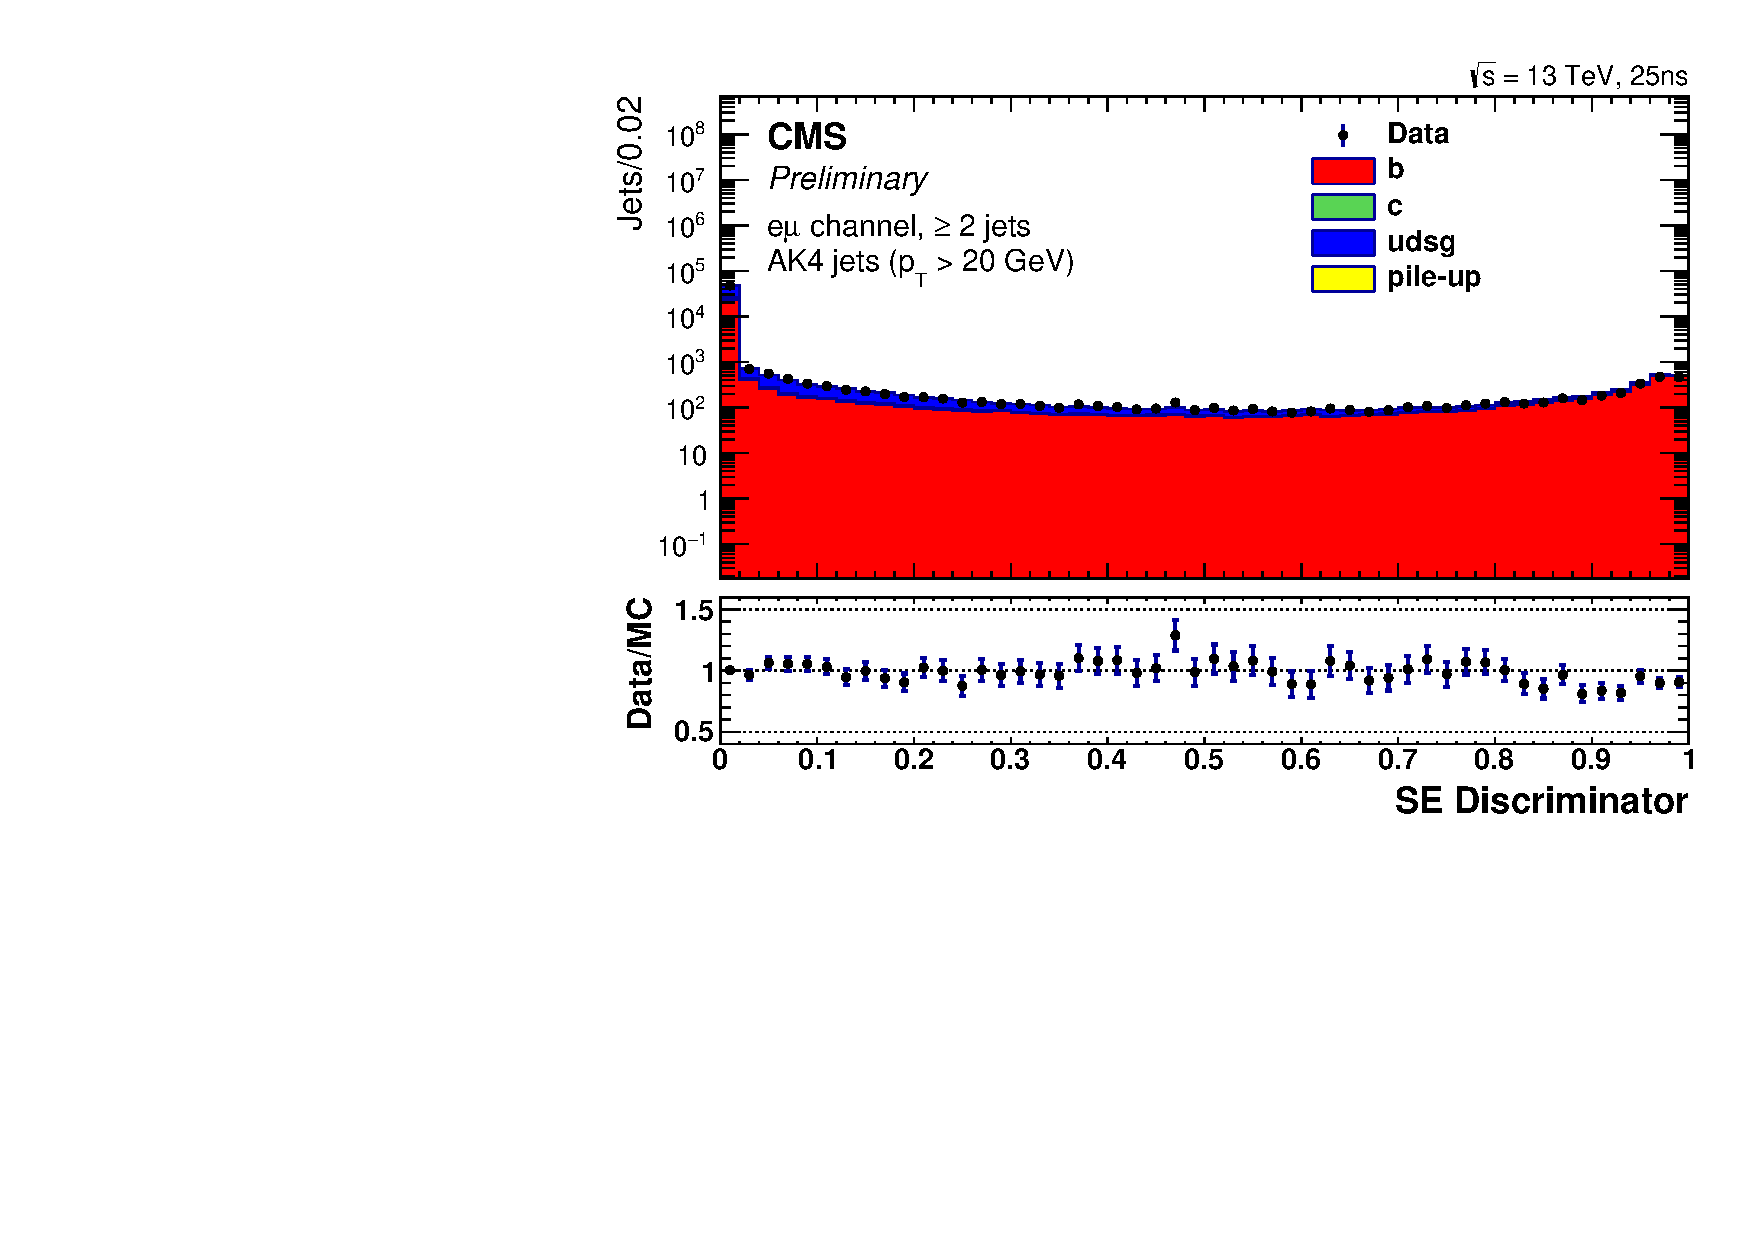
\includegraphics[width=0.5\textwidth]{figures/btv/softel.pdf}}
\subfloat[The soft muon b~tagger]{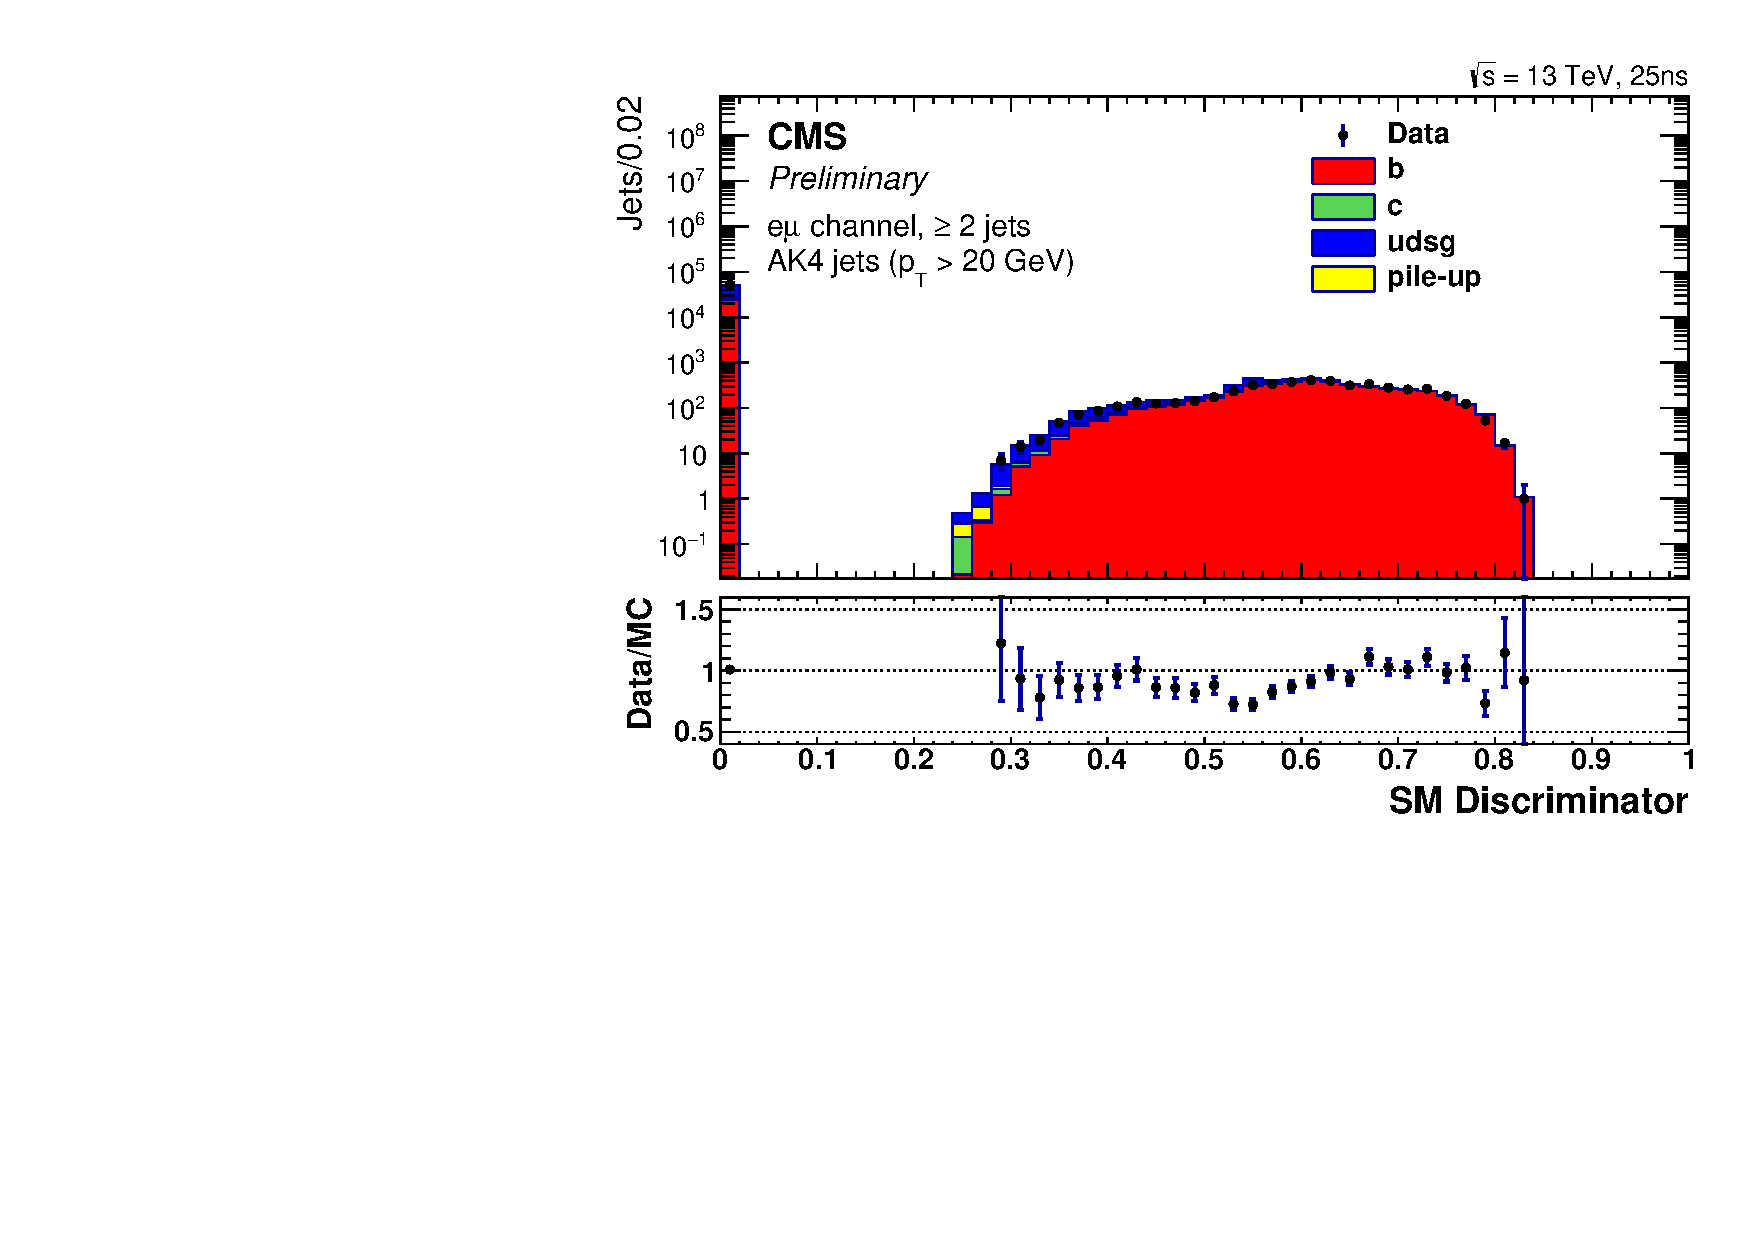
\includegraphics[width=0.5\textwidth]{figures/btv/softmu.pdf}} \\
\caption[The soft lepton b discriminator distributions]{The discriminator distributions of the soft lepton b taggers in dileptonic ($\mathrm{e\mu}$) \ttbar+jets events. The large fraction of jets with a soft muon discriminator value around 0 arises from cases where no muon was associated to the jet. Figures from~\cite{CMS-PAS-BTV-15-001}.}
\label{fig:btag_softlep}
\end{centering}
\end{figure}

\subsubsection{The CSVv2 b~tagger}
The Combined Secondary Vertex algorithm V2 (CSVv2) is based on the original CSV implementation introduced in Run I~\cite{Chatrchyan:2012jua} and uses machine learning to combine track and secondary vertex information such as vertex mass or flight distance. Based on the presence and quality of the secondary vertex, the CSVv2 is optimised in several categories:
\begin{itemize}
\item presence of a good secondary vertex, in which case the flight distance and other vertex related variables are defined
\item the pseudo-vertex category with two good tracks but no vertex fit, in which case the track parameters are used
\item a no vertex category that uses information only from displaced tracks.
\end{itemize}
The final CSVv2 discriminant is a likelihood combination of binary classifiers based on artificial neural networks with a single hidden layer in all 3 categories. The CSVv2 algorithm has been deployed on both the AVR vertices as CSVv2 (AVR) and the IVF vertices, denoted CSVv2 (IVF). The CSVv2 (IVF) has an efficiency of about~$66\%$~for b jets at a mistag rate for light jets (udsg-associated) of about~$1\%$~based on~\ttbar~simulation at the CSVv2 medium working point~\cite{CMS-PAS-BTV-15-001}. The CSVv2 b~discriminator is the primary b~tagging algorithm used in the end of Run I and the beginning of Run II at CMS. The discriminator distributions are shown on~\cref{fig:btag_csv}.

\begin{figure}
\begin{centering}
\subfloat[The CSVv2 AVR b~tagger]{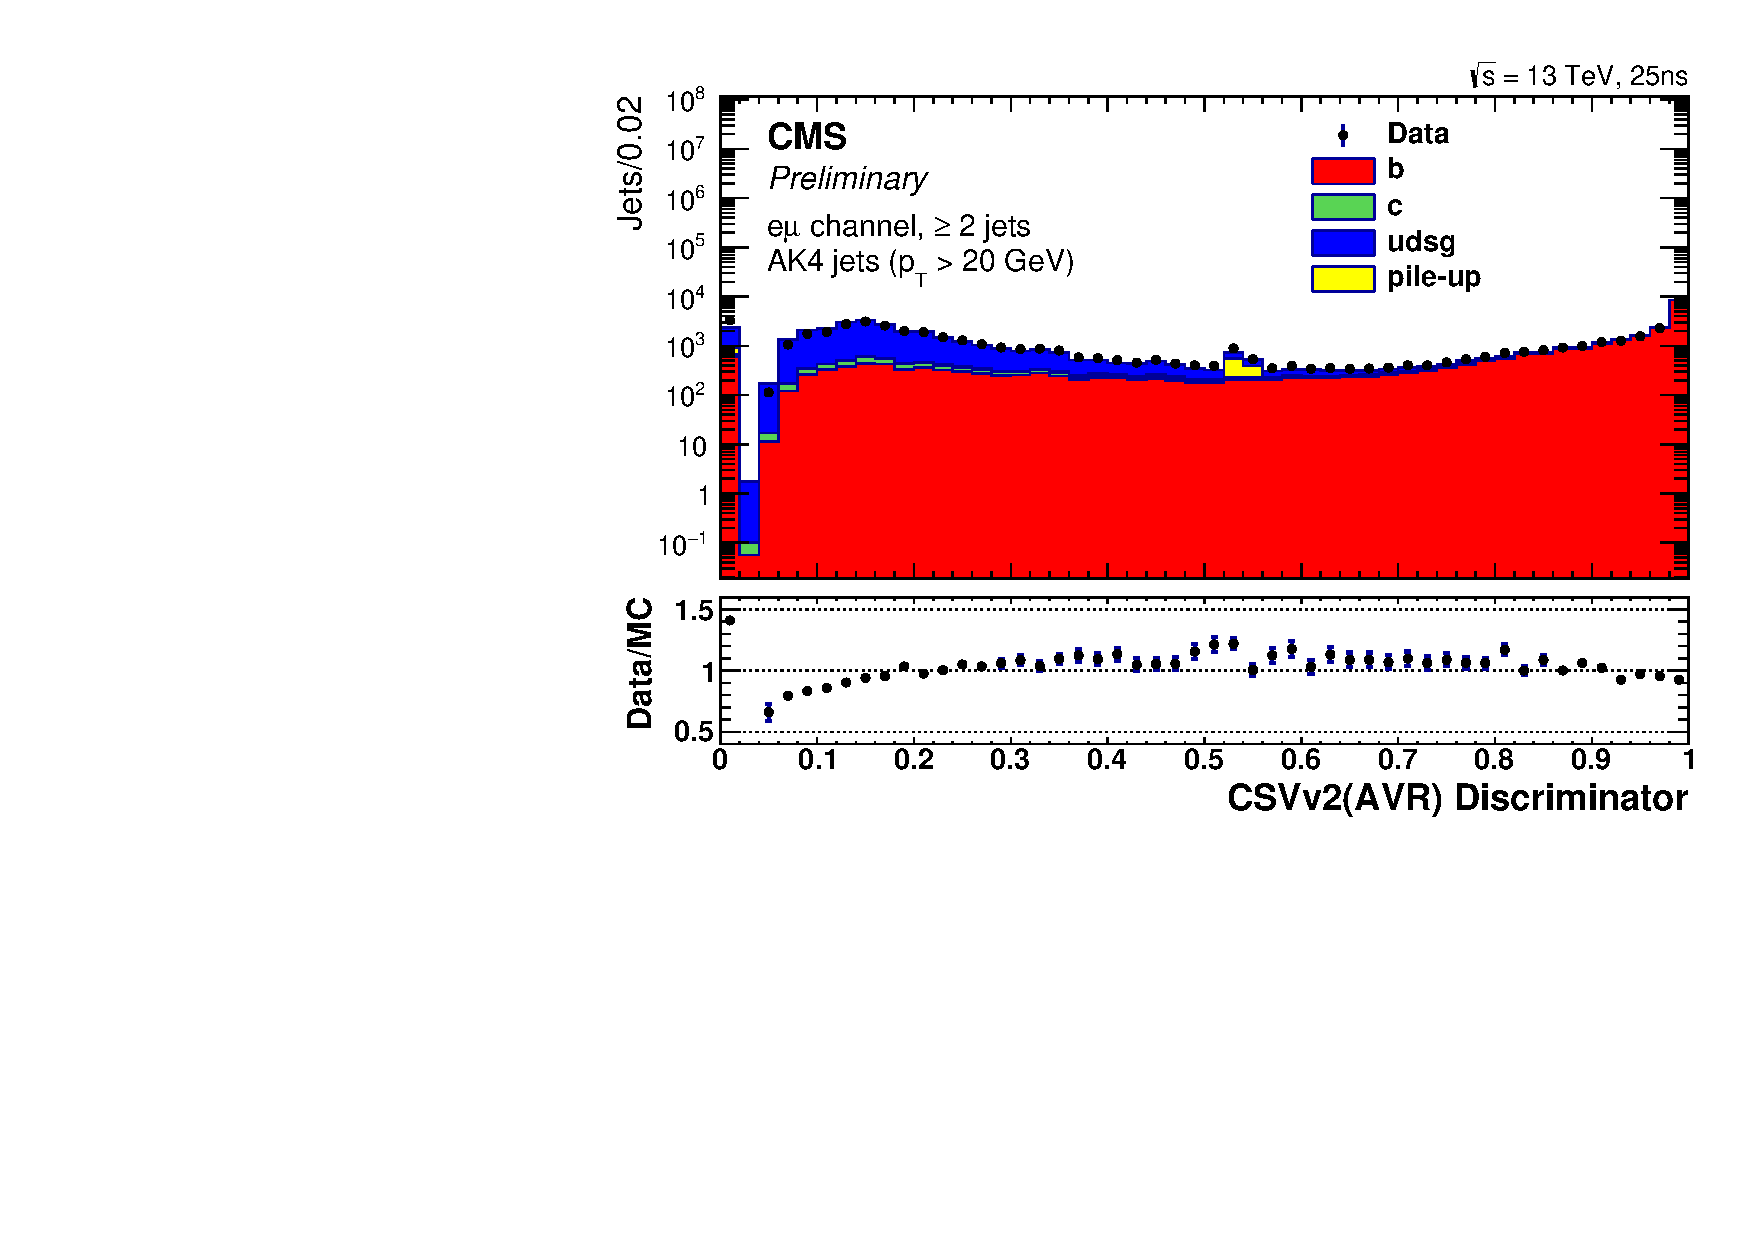
\includegraphics[width=0.5\textwidth]{figures/btv/csvavr.pdf}}
\subfloat[The CSVv2 IVF b~tagger]{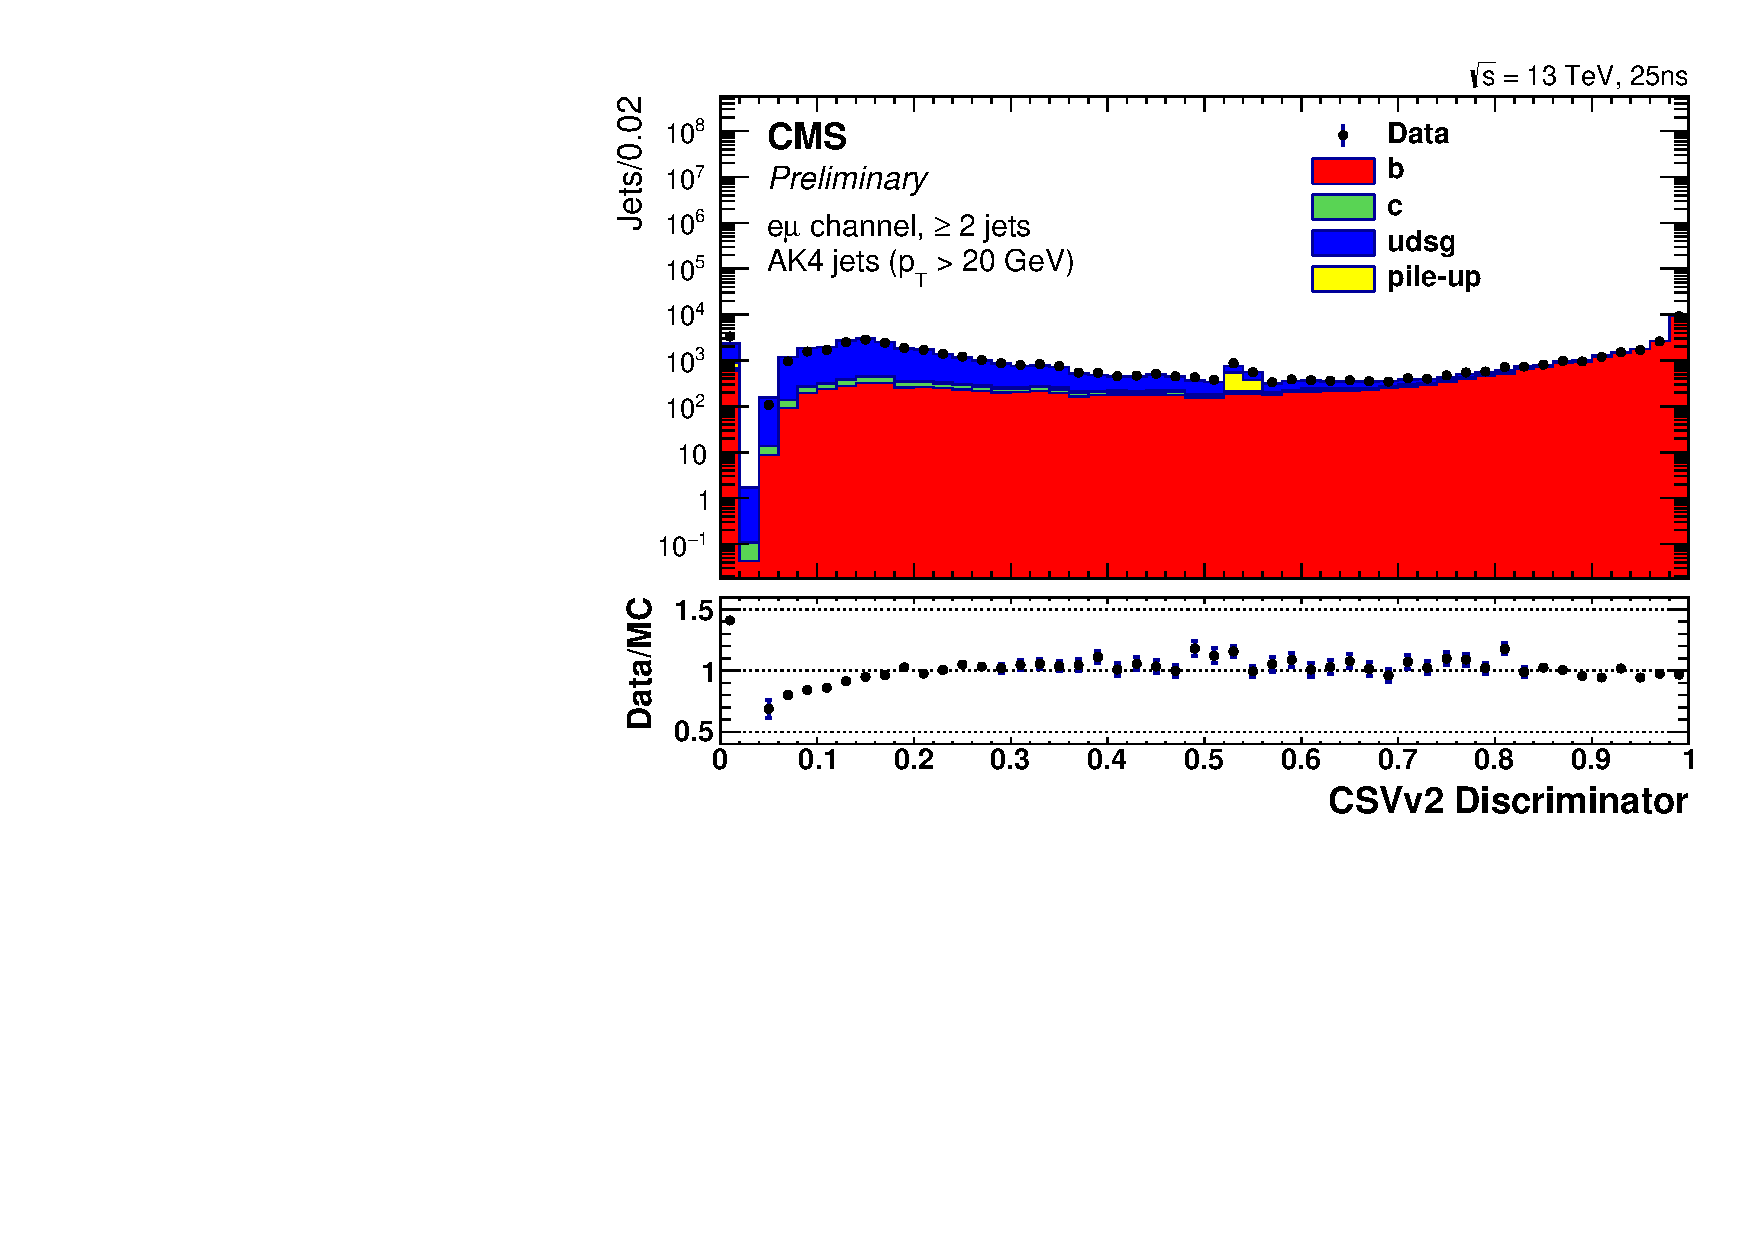
\includegraphics[width=0.5\textwidth]{figures/btv/csvivf.pdf}} \\
\caption[The CSVv2 b~tagger discriminator distributions]{The discriminator distributions of the CSVv2 b~taggers in dileptonic ($\mathrm{e\mu}$) \ttbar+jets events. Figures from~\cite{CMS-PAS-BTV-15-001}.}
\label{fig:btag_csv}
\end{centering}
\end{figure}

\section{The combined multivariate b~tagger}
In Run II, we have developed an improved b~tagger algorithm for CMS that combines the aforementioned individual b~taggers, relying on various sources of information, to a single discriminator using boosted decision trees (BDTs) via the \texttt{scikit-learn} package~\cite{scikit-learn}. This combined discriminator, denoted cMVAv2, exploits the fact that the AVR and IVF vertex reconstruction algorithms may reconstruct different vertices, the presence or lack of soft leptons and secondary vertex information simultaneously. The tagger is optimised on~\ttbar+jets simulation, with cross-validation on a multi-jet simulation sample. At a similar b-jet efficiency to the CSVv2 medium working point ($\epsilon_b \simeq 70\%$), the cMVAv2 b-tagger algorithm reduces the mistag rate for light jets from~$1\%$~to about~$0.5\%$, as seen on~\cref{fig:btag_roc}.

\begin{figure}
\begin{centering}
\subfloat[The b~tagging and misclassification probability.]{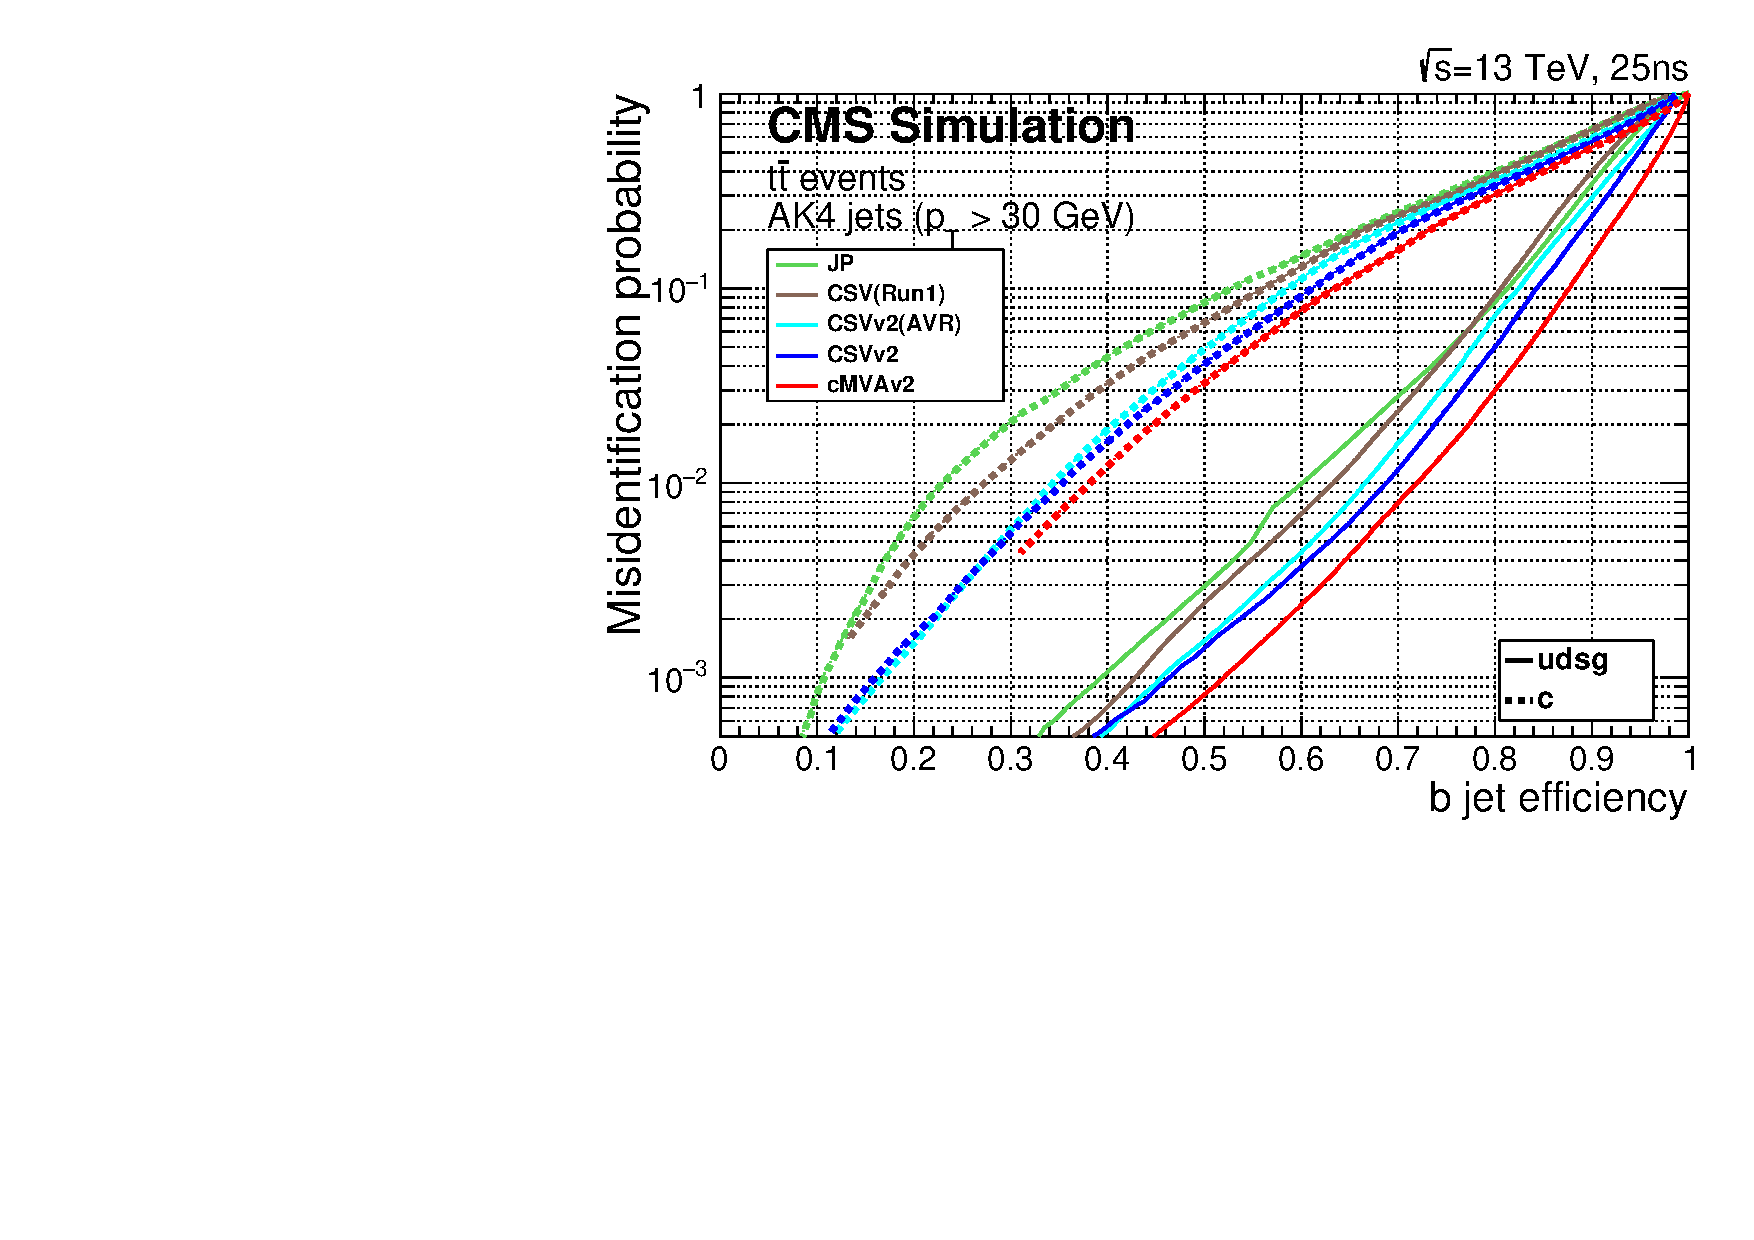
\includegraphics[width=0.5\textwidth]{figures/btv/Figure_008.pdf}}
\subfloat[The discriminant distribution for the cMVAv2 discriminator.]{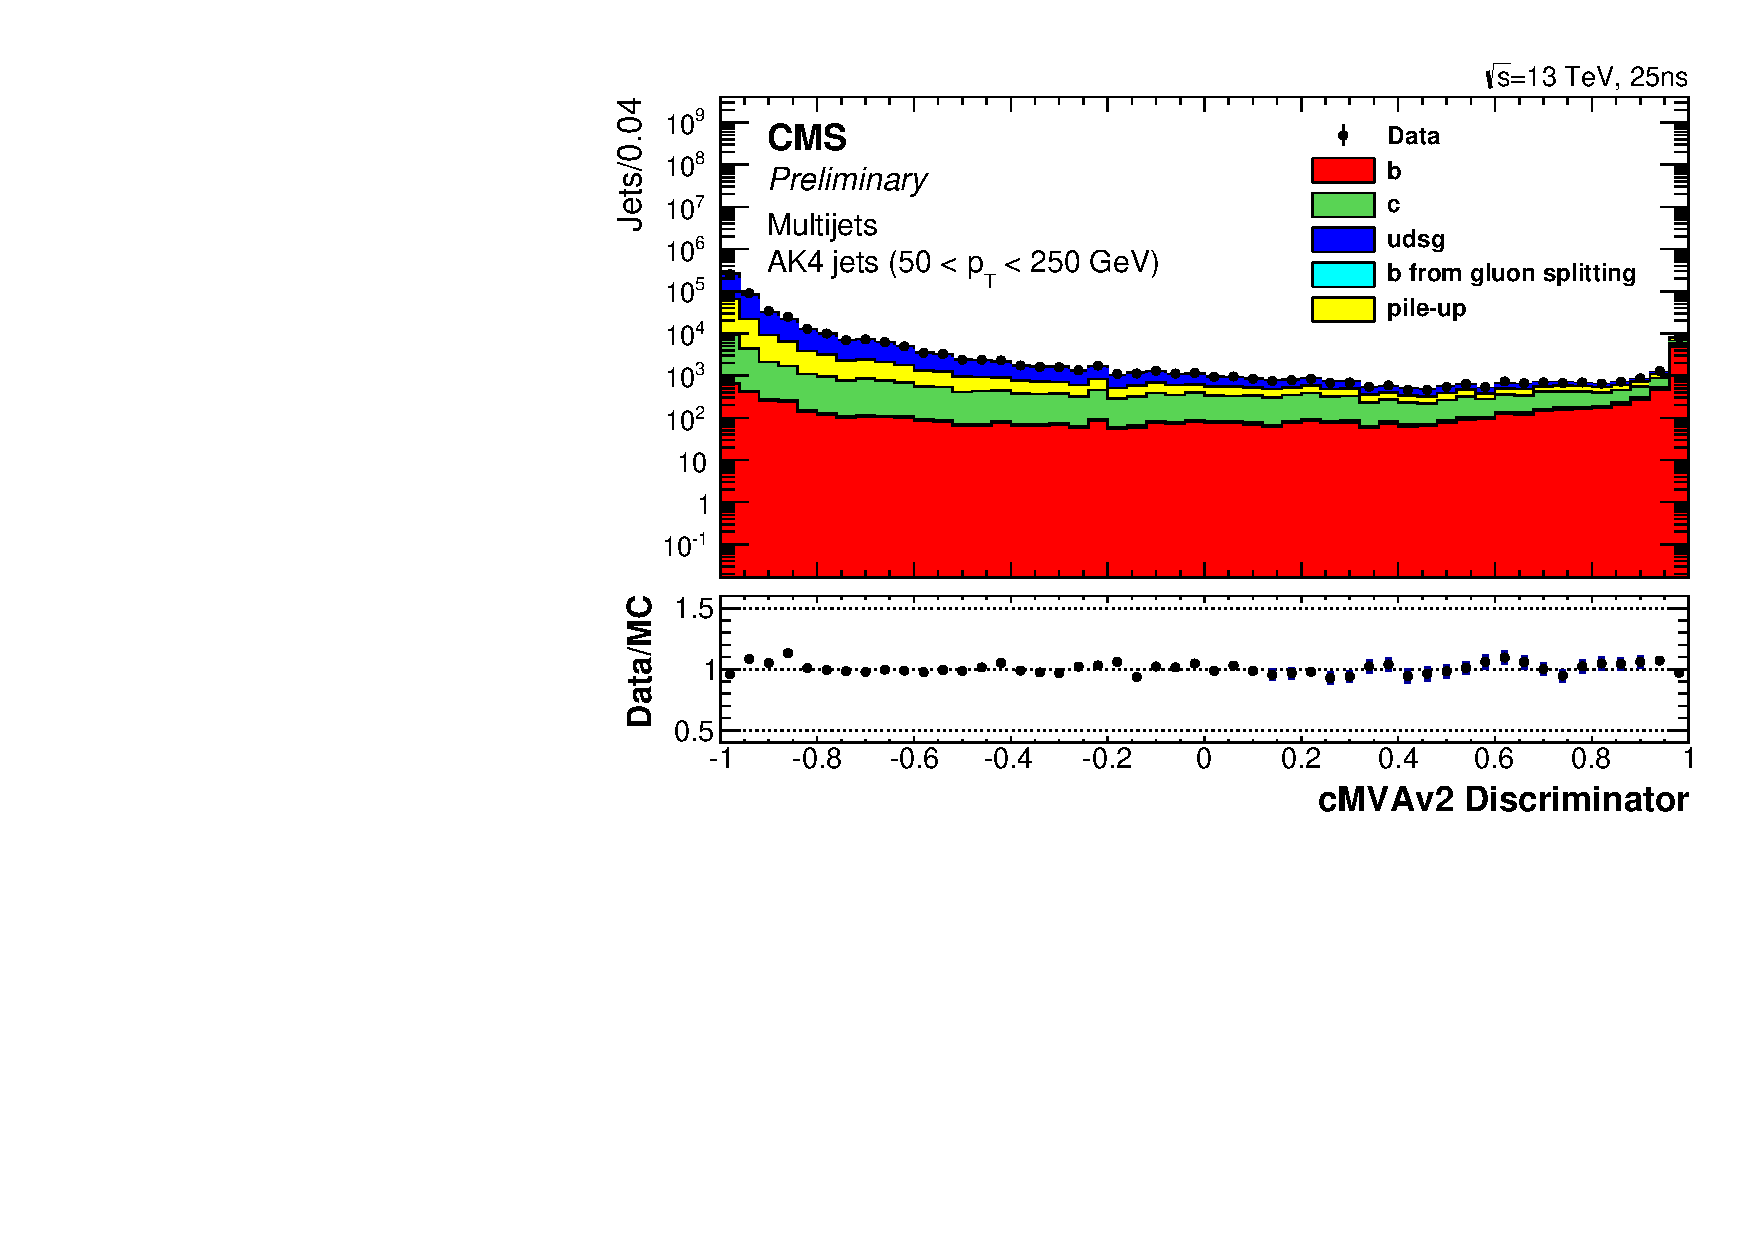
\includegraphics[width=0.5\textwidth]{figures/btv/Figure_007-a.pdf}} \\
\caption[The performance of the CMS b~taggers in Run II]{The performance of the CMS b~taggers in Run II. On~(\textbf{a}), the efficiency to correctly tag b~jets is shown with respect to the misclassification probability for light jets (udsg-associated, solid line) and charm jets (dashed line), based on~\ttbar+jets simulation. The medium working point correspond to a light jet efficiency of $\epsilon_{l} = 1\%$ and we see that the cMVAv2 b discriminator has~$\epsilon_{b} \simeq 72\%$, compared to the CSVv2 b-efficiency~$\epsilon_{b} \simeq 66\%$. On~(\textbf{b}), we show the comparison of the cMVAv2 discriminator between data and simulation, where data-driven scale factors are applied. Figures from~\cite{CMS-PAS-BTV-15-001}}
\label{fig:btag_roc}
\end{centering}
\end{figure}

\subsection{Implementation}
The cMVAv2 b~discriminator is a optimised as a binary classifier in a supervised training mode on jets derived from~\ttbar+jets simulation. Simulated jets are assigned a flavour by re-clustering the jet with momentum-scaled generator-level hadrons in such a way that the momentum of the jet is not altered. Based on the clustered hadrons, a jet is assigned to be a b jet, a c jet or a light jet in decreasing priority. We use particle flow jets with~$p_T > 20$~GeV,~$|\eta| < 2.5$~and enhance the selected jet sample at high~$p_T$~and~$|\eta|$~by limiting the amount of jets in the binned 2D distribution of~$p_T \in [20, 620], |\eta| \in [0, 2.5]$~with 100 bins per dimension to~$N_{\mathrm{max}} = 10000$~per bin. This sub-sampling technique effectively gives higher weight to the tails of the momentum and pseudorapidity distribution and reduces the simulated data to an amount that fits in the RAM of a conventional PC. We use an inclusive~\ttbar+jets sample generated with~\powheg~and \pythia~and an independent multi-jet sample generated with~\pythia~for cross-validation. We list the details of the simulated samples in~\cref{tab:btag_samples}.

\begin{table}[h!]
\begin{center}
\begin{tabular}{c|cccc}
\hline
MC sample & events & b jets & c jets & light jets \\
\hline
\ttbar+jets & 28M & 9.5M & 3.7M & 11M \\
multi-jet (QCD) & 29M & 1.2M & 2.3M & 17M \\
\hline
\hline
\end{tabular}
\caption[The training and validation samples for cMVAv2]{The simulated samples used for optimising and validating the cMVAv2 b~tagger. The jets are filtered with a~$p_T, |\eta|$-dependent selection that restricts the amount of jets in the high-statistics, low~$p_T$~and~$|\eta|$~part of the distribution.}
\label{tab:btag_samples}
\end{center}
\end{table}

\subsubsection{Kinematic reweighting}
Since the kinematic distributions in~$p_T$~and~$|\eta|$~of b, c and light jets are different due to their different production modes, we need to ensure that the b~tagger algorithm distinguishes between jets of different flavour based on quantities that are mostly independent of kinematics. In addition to the subsampling technique mentioned above, we reweight the jet sample used in the training of the binary classifier such that the distributions are roughly uniform in~$p_T$~and~$\eta$~using a weight~$w(p_T,|\eta|,\mathrm{flavor})$~derived on simulation, as shown on~\cref{fig:btag_pt_reweight}. This reweighting does not have a significant effect on the overall final b~tagging performance of the discriminator, however, it helps to make the optimisation less sample-dependent.

\begin{figure}
\begin{centering}
\subfloat[The jet~$p_T$~distributions by flavor.]{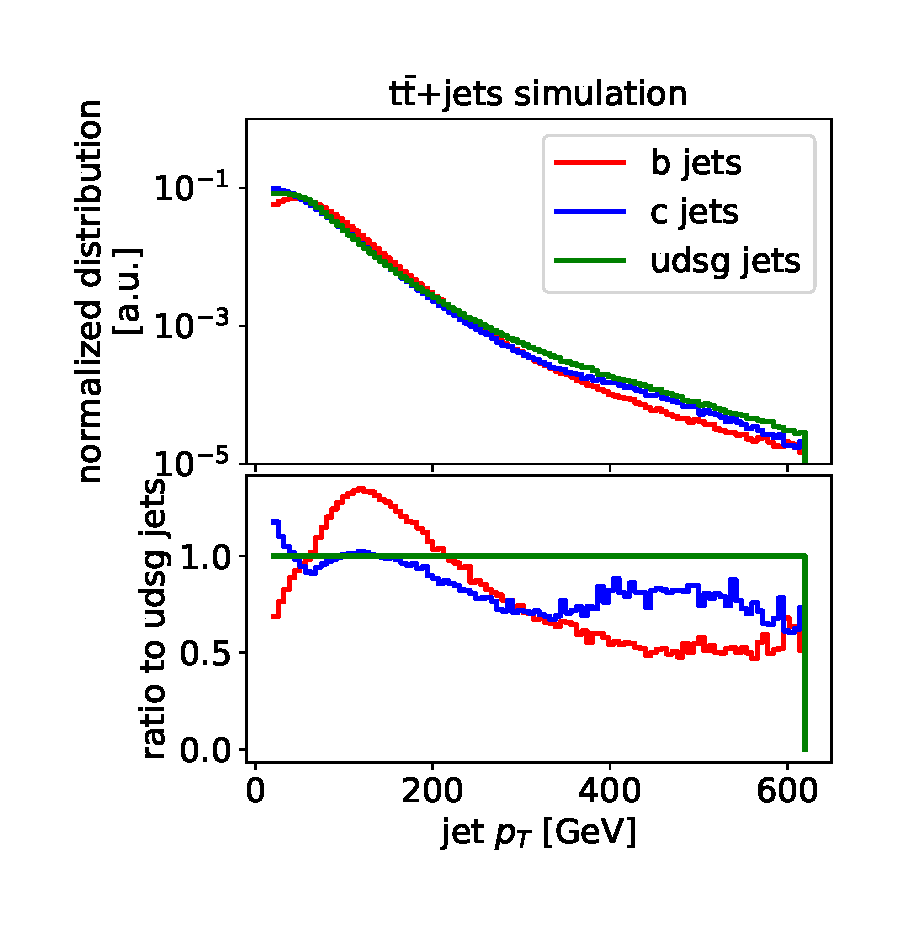
\includegraphics[width=0.5\textwidth]{figures/btv/jet_pt_flavor.pdf}}
\subfloat[The reweighted jet~$p_T$~distribution.]{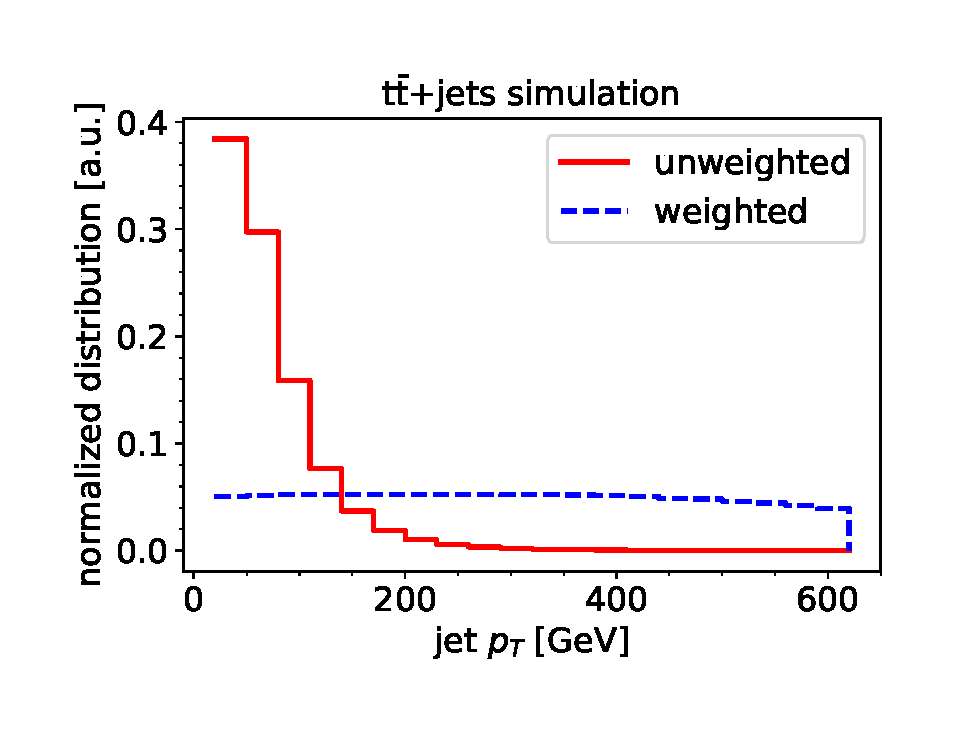
\includegraphics[width=0.5\textwidth]{figures/btv/jet_pt_weighted.pdf}} \\
\caption[Comparison of jet kinematics in MC simulation by jet flavour]{Comparison of jet kinematics by associated MC flavour before and after the kinematic reweighting. On~(\textbf{a}), we compare the jet~$p_T$~distributions for b, c and light jets. We see that b jets have a momentum distribution that is narrower and peaks around~100~GeV. On~(\textbf{b}), we show the jet~$p_T$~distribution before and after applying the kinematic reweighting~$w(p_T,|\eta|,\mathrm{flavor})$. We see that the reweighted distribution is roughly uniform, with small differences caused by simulation statistics in the derivation of the weight. These distributions are derived using~\ttbar+jets simulation.}
\label{fig:btag_pt_reweight}
\end{centering}
\end{figure}

\subsubsection{Input variables}
We have used the b~tagger algorithms described earlier as inputs to the cMVAv2 algorithm. In particular, we use the following 6 b~discriminators: CSV~(AVR), CSV~(IVF), JP, JBP, SoftMuon and SoftElectron. We have studied the correlation between CSV~(AVR) and CSV~(IVF), as shown on~\cref{fig:btag_csv_correlation}. Although the linear correlation coefficient is around~$C \simeq 0.9$~for all flavours, we see a non-negligible contribution from jets which have different vertices from the two vertexing algorithms and thus different CSV discriminator values. Therefore, we expect that a combined discriminator will outperform either of the two. Furthermore, the information provided by the JP and JBP discriminators can complement the CSV in cases no vertices could be found. To verify whether adding the additional input b~discriminators provides useful information for b~tagging, we optimise a set of BDT classifiers iteratively by including the 6 input discriminators one by one.

\begin{figure}
\begin{centering}
\subfloat[bottom jets]{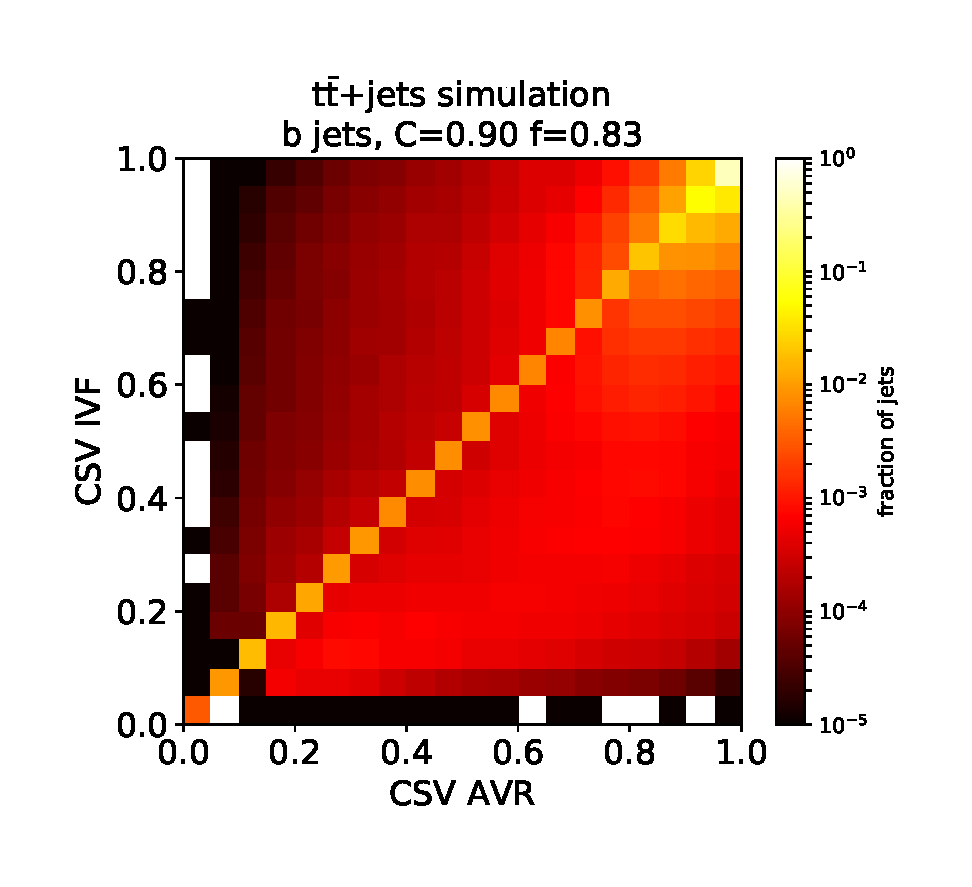
\includegraphics[width=0.35\textwidth]{figures/btv/CSV_AVR_IVF_corr_b.pdf}}
\subfloat[charm jets]{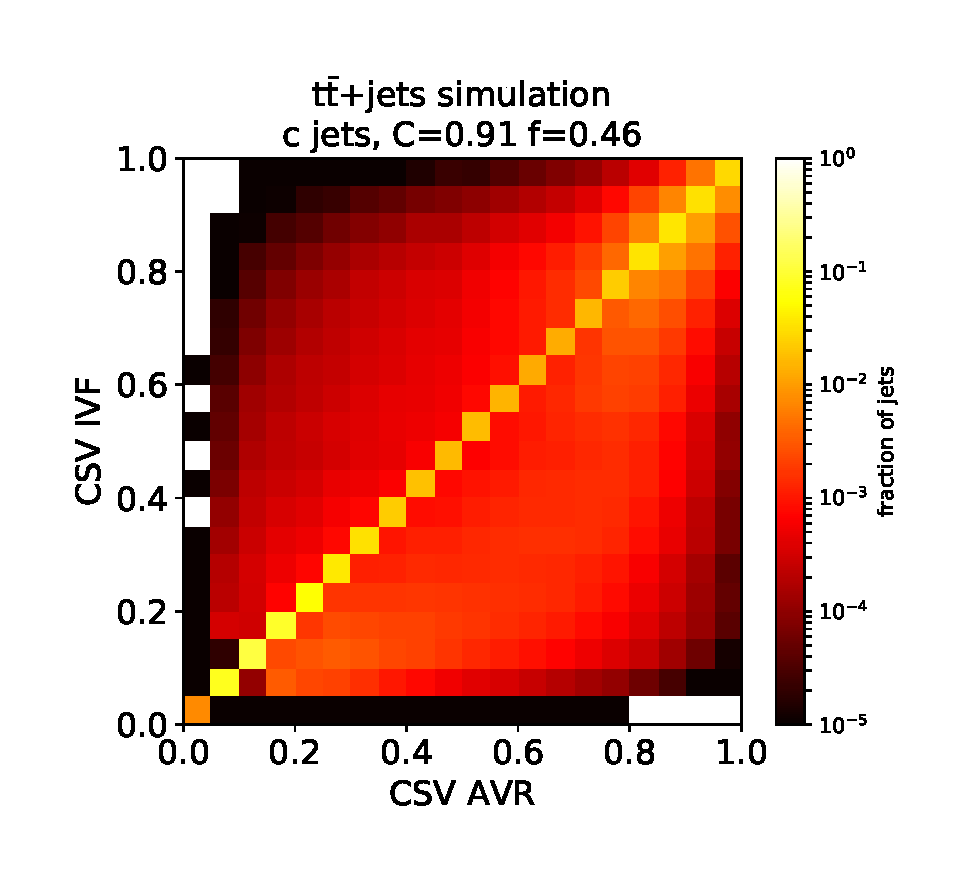
\includegraphics[width=0.35\textwidth]{figures/btv/CSV_AVR_IVF_corr_c.pdf}}
\subfloat[light~(udsg) jets]{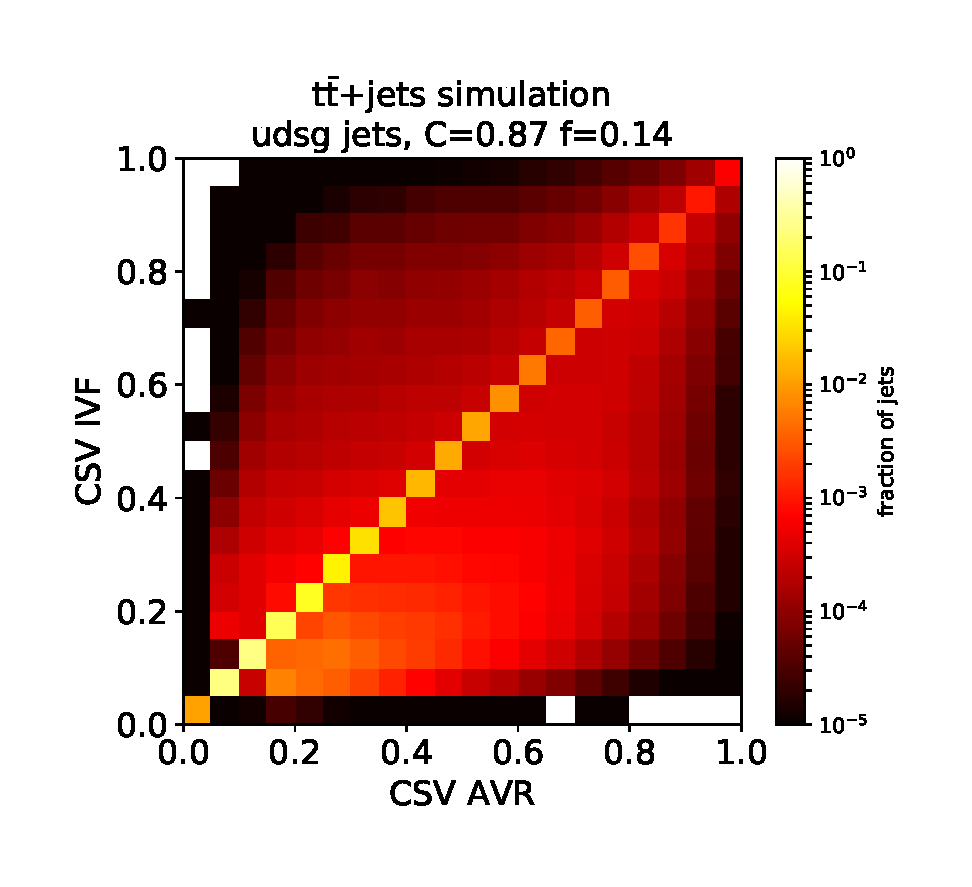
\includegraphics[width=0.35\textwidth]{figures/btv/CSV_AVR_IVF_corr_l.pdf}} \\
\caption[The correlation between the CSV b~discriminator value using AVR and IVF vertices]{The correlation between the CSV b~discriminator value using AVR and IVF vertices. Despite the high linear correlation coefficient~$C$, we see a significant fraction of jets~$f$~with non-equal values of the two discriminators, visible as the non-diagonal elements in the 2D distribution. These distributions are derived using the~\ttbar+jets~simulation.}
\label{fig:btag_csv_correlation}
\end{centering}
\end{figure}

\subsection{optimisation and validation}
In order to convince ourselves of the BDT optimisation, we perform a number of validation steps. The optimisation and validation of the BDTs is done on statistically independent subsets of the~\ttbar~+jets simulation sample and the statistical over-training is negligible after 200 boosting iterations, as can be seen on~\cref{fig:btag_loss}. This is due to the large amount ($\mathcal{O}(10^7)$ jets) of available simulation statistics, combined with the input variable space being relatively low-dimensional~($N=6$). We have further validated the training using $k$-fold cross-validation, where the training is repeated $k$ times on sub-samples of the data, and found the statistical uncertainty between sub-samples to be negligible.

\begin{figure}
\begin{centering}
\subfloat[The loss function (top) with respect to boosting iteration and the difference between training and validation loss (bottom).]{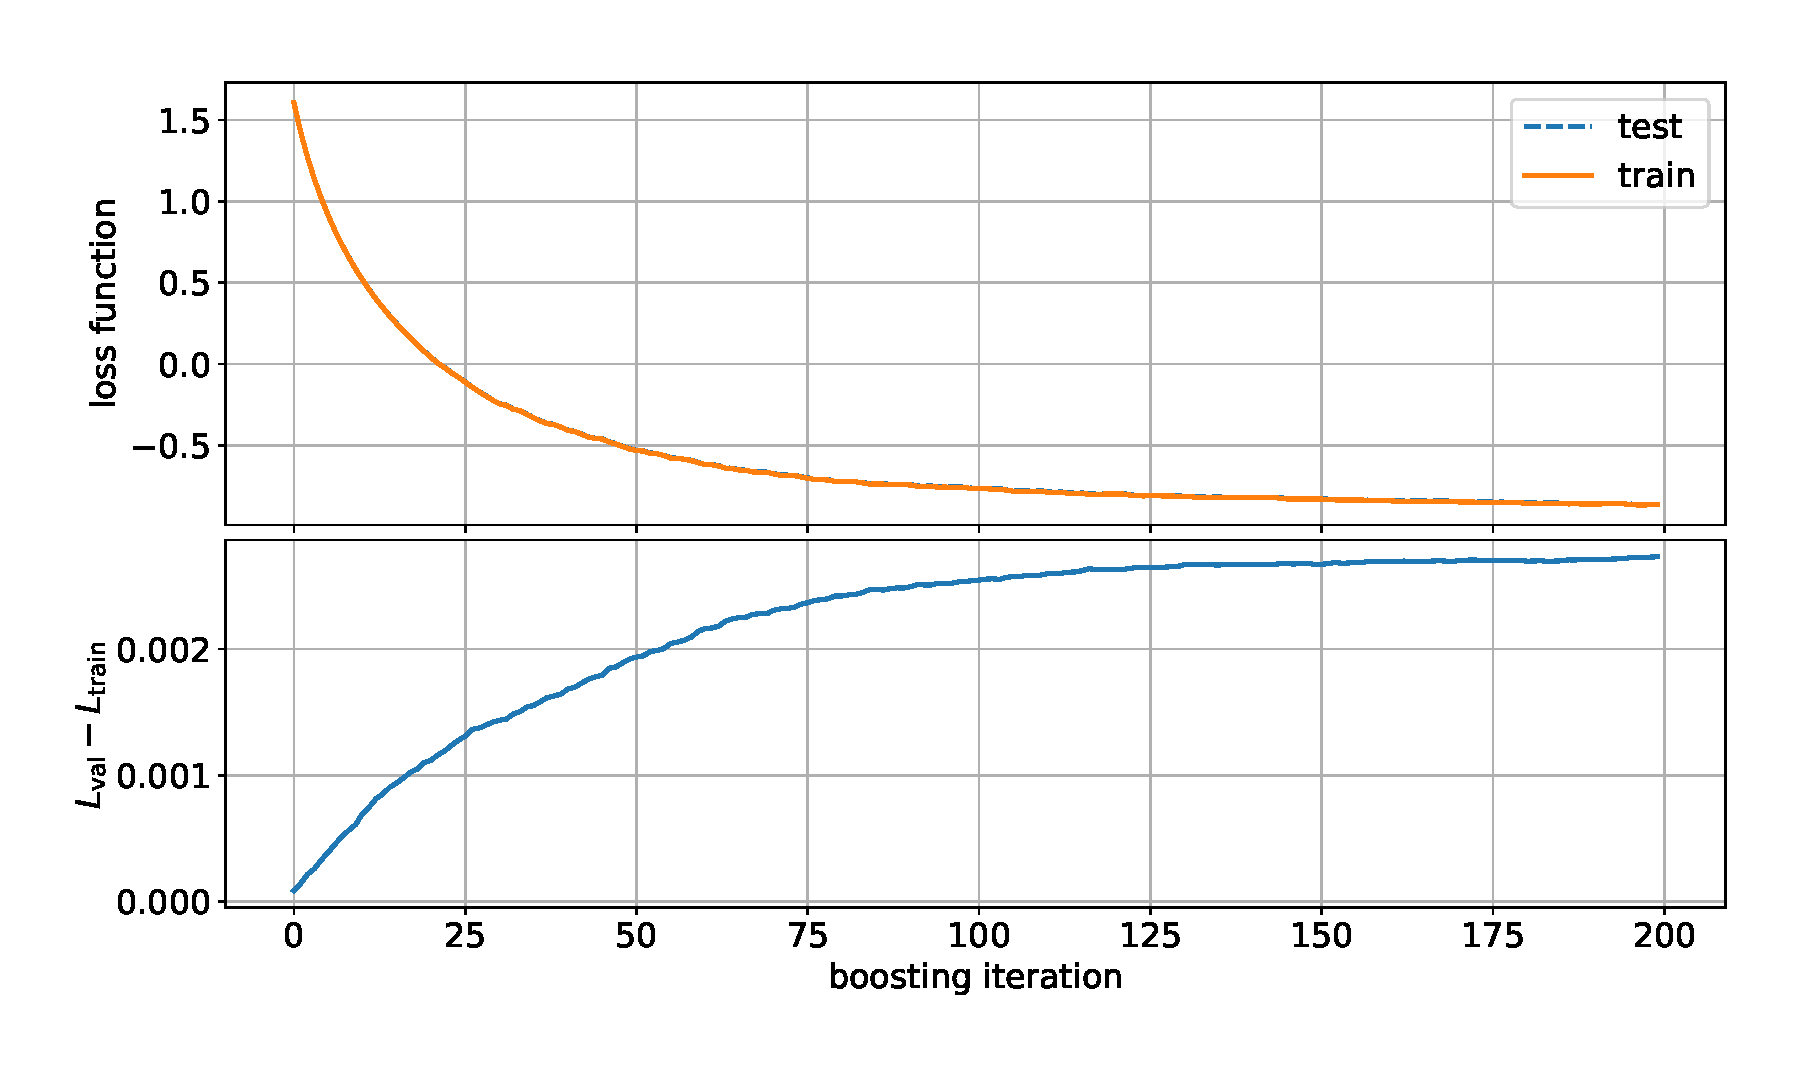
\includegraphics[width=0.7\textwidth]{figures/btv/loss.pdf}} \\
\subfloat[Ratio of discriminator distributions.]{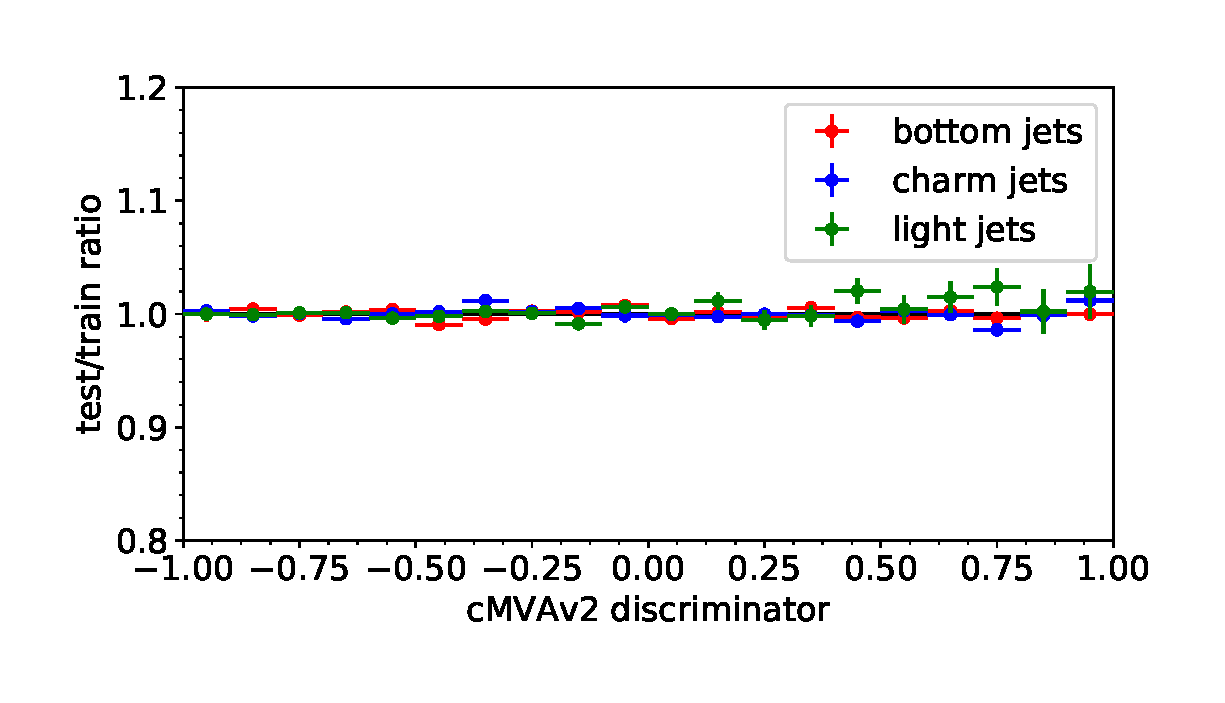
\includegraphics[width=0.7\textwidth]{figures/btv/train_test_distribution.pdf}}
\caption[The cMVAv2 BDT loss as a function of boosting iteration]{Validation of the cMVAv2 against over-training by comparing the loss function between the training set and the statistically independent validation set as a function of the boosting iteration on~(\textbf{a}). We see good convergence after~$N=200$~boosting steps, with a negligible difference between the loss functions. Furthermore, on~(\textbf{b})~we compare the discriminator distributions on the training and test sets, with the ratio being compatible with unity within statistical uncertainties.}
\label{fig:btag_loss}
\end{centering}
\end{figure}

We analyse the performance of the optimised b~discriminator in terms of the efficiency for selecting b jets~(signal) with respect to charm and light jets~(background). On~\cref{fig:btag_cmva_roc}, we show the ROC AUC performance metric of the various stages of cMVAv2 optimisation. In general, we see that the BDTs are able to take advantage of all the input taggers, with the inclusion of each input improving the overall discrimination power monotonically. The optimisation is carried out on the~\ttbar~+jets simulation sample and we have cross-checked the results against the multi-jet simulation, where we have seen an equivalent improvement.

\begin{figure}
\begin{centering}
\subfloat[b vs light jets]{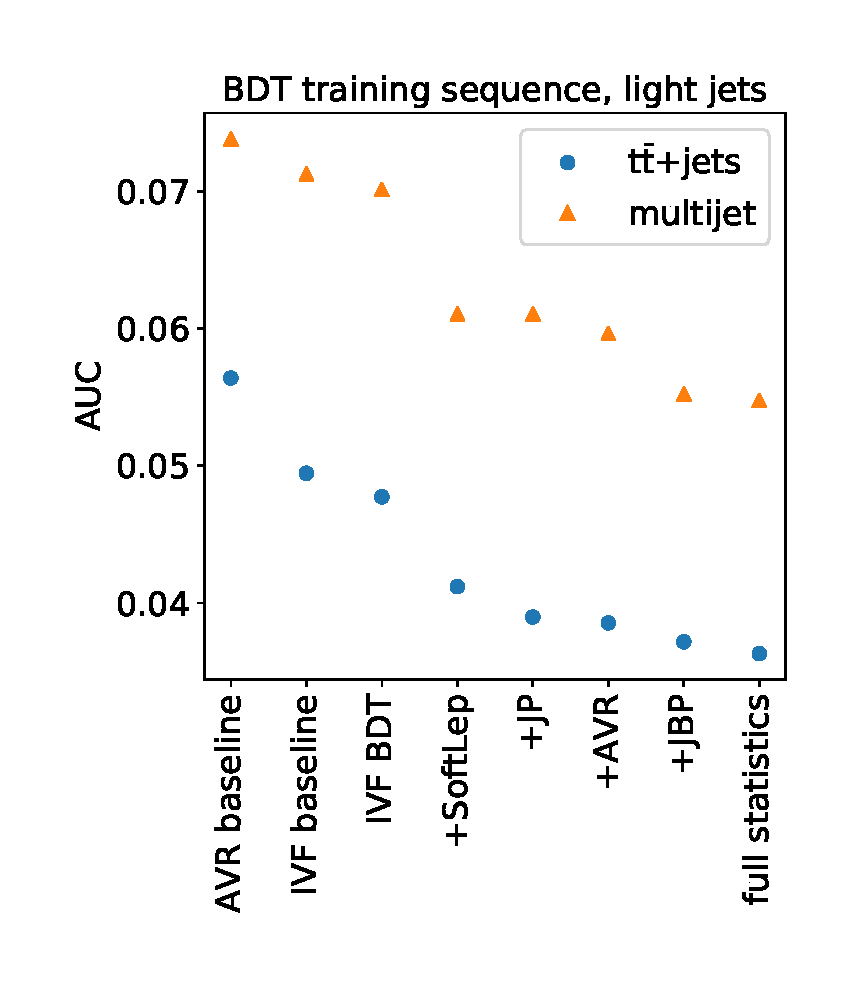
\includegraphics[width=0.5\textwidth]{figures/btv/bdt_seq_light.pdf}}
\subfloat[b vs charm jets]{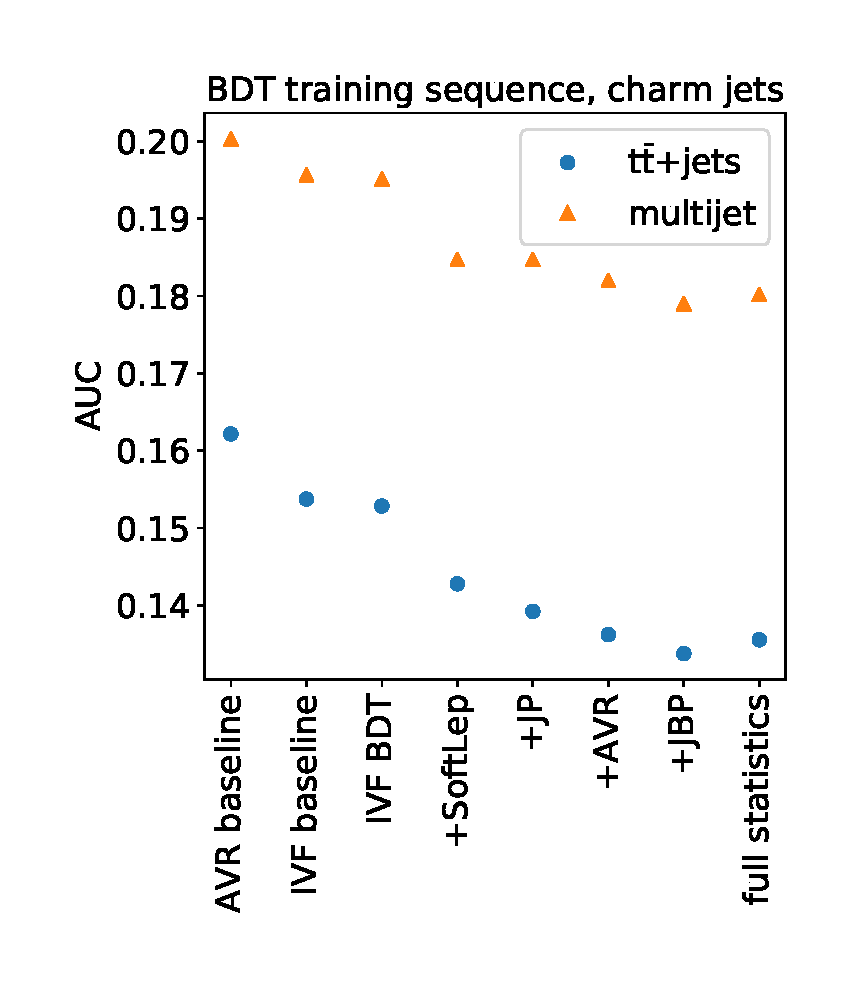
\includegraphics[width=0.5\textwidth]{figures/btv/bdt_seq_charm.pdf}} \\
\caption[The cMVAv2 performance as a function of training variables.]{The performance characteristic ROC AUC as a function of the number of variables included in the BDT training, where lower values correspond to better discrimination. The baseline CSV b~discriminators with IVF and AVR vertices are compared to the cMVAv2, which is optimised by successively including the IVF, SoftLepton, JP, AVR, JBP taggers with partial training statistics. We see that the inclusion of the Soft Muon and Soft Electron b~taggers provides a significant improvement to the b jet vs. light jet discrimination (\textbf{a}), as well as b jet vs. charm jet (\textbf{b}). The best discrimination against light jets is reached by using the full simulation sample. We have performed the optimisation on the~\ttbar~+jets simulation sample, and cross-checked the results on the multi-jet sample. Statistical uncertainties on the performance are verified using cross-validation and are negligible.}
\label{fig:btag_cmva_roc}
\end{centering}
\end{figure}

The performance of the optimised cMVAv2 b~discriminator is validated by comparing the efficiency of selecting light jets or charm jets as b~tagged at a fixed b~tagging efficiency for b~jets as a function of jet kinematics, as shown on~\cref{fig:btag_kinematics}. We see that the cMVAv2~b~discriminator has somewhat more stable performance with respect to jet kinematics than the CSV b~discriminators and an improved discrimination power in the forward region $|\eta| > 1.5$. The cMVAv2~b~discriminator uniformly outperforms the CSV algorithm over the studied jet momentum range $20 < p_T < 320$,~$0 < |\eta| < 2.5$. Overall, the cMVAv2 algorithm has a mistagging efficiency lower by at least~$20\%$~($10\%$) for light jets (charm jets) over the full range.

\begin{figure}
\begin{centering}
\subfloat[light jet efficiency in $p_T$]{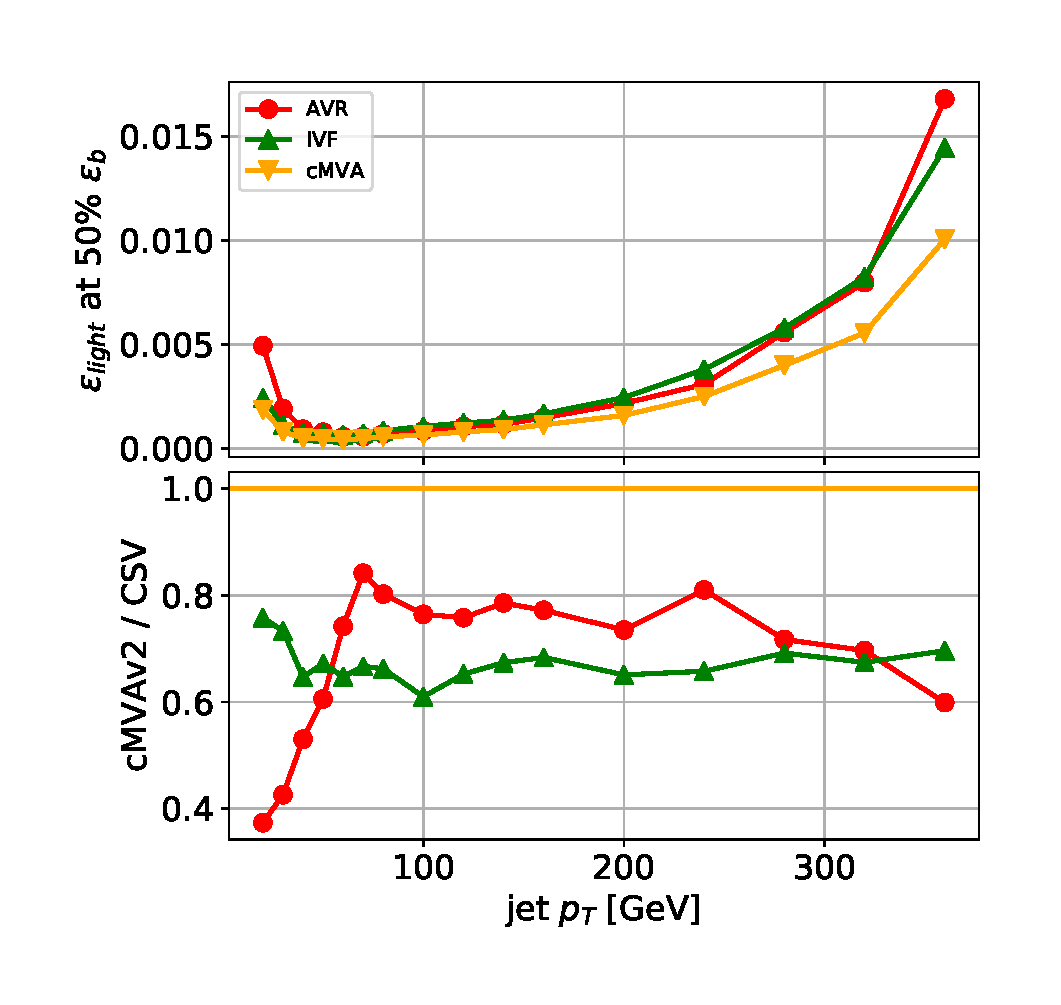
\includegraphics[width=0.5\textwidth]{figures/btv/tt_e50_l_pt.pdf}}
\subfloat[light jet efficiency in $|\eta|$]{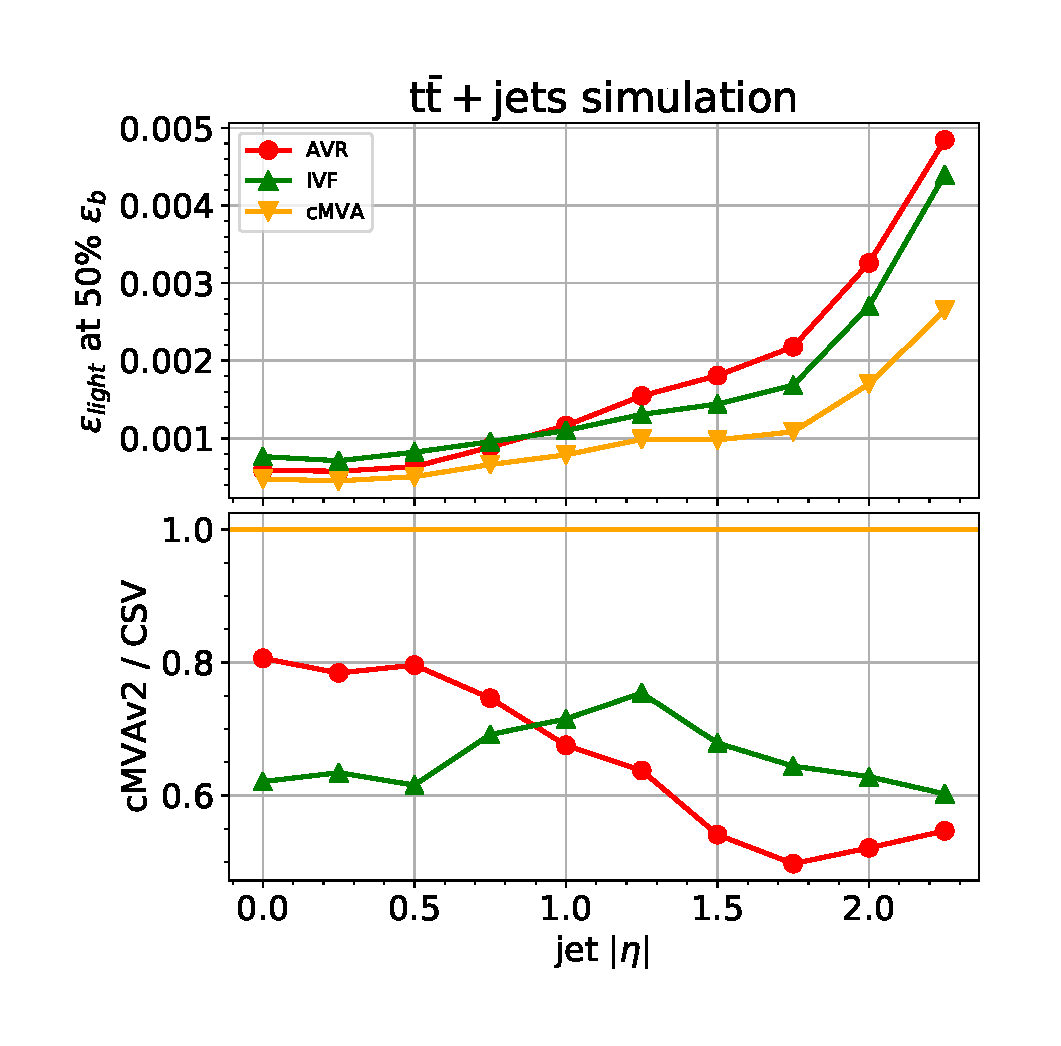
\includegraphics[width=0.5\textwidth]{figures/btv/tt_e50_l_eta.pdf}} \\
\subfloat[charm jet efficiency in $p_T$]{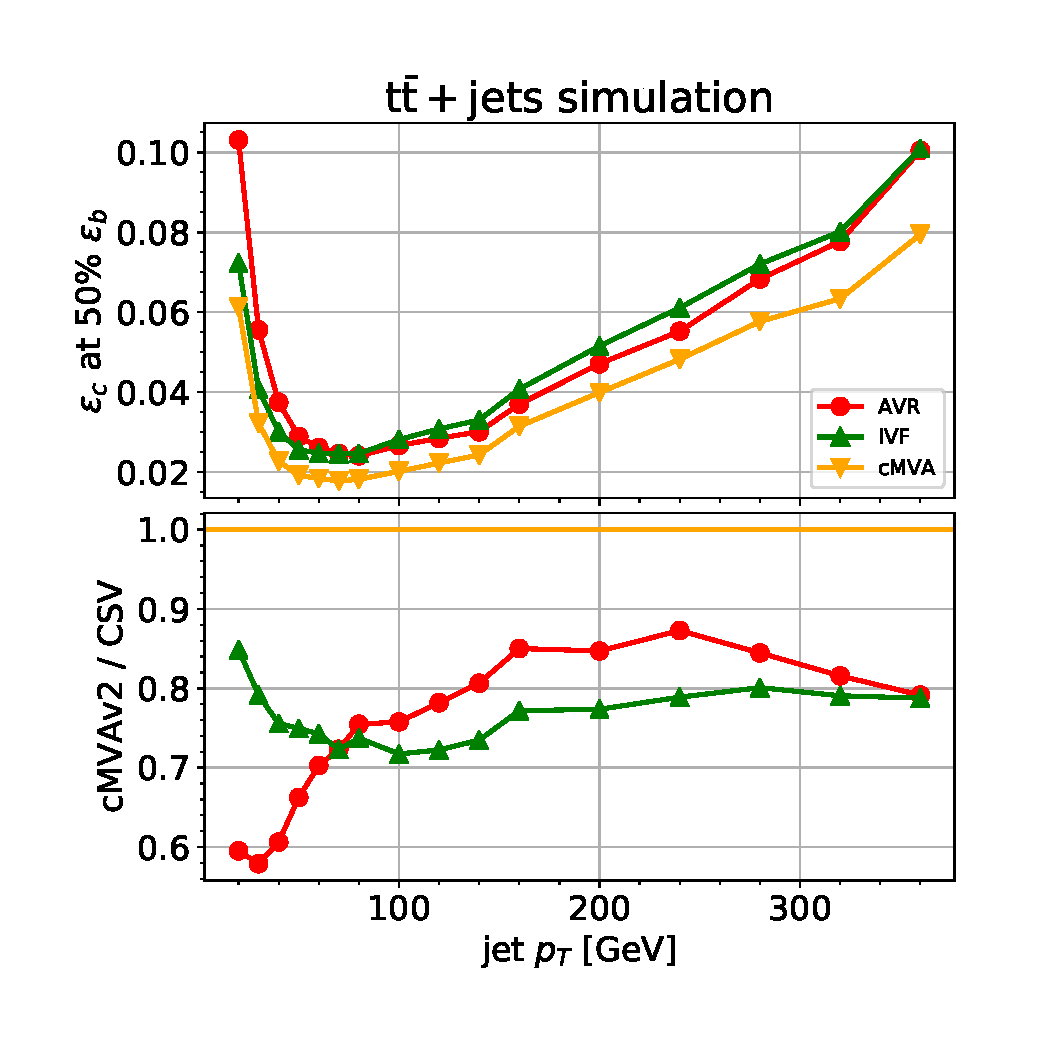
\includegraphics[width=0.5\textwidth]{figures/btv/tt_e50_c_pt.pdf}}
\subfloat[charm jet efficiency in $|\eta|$]{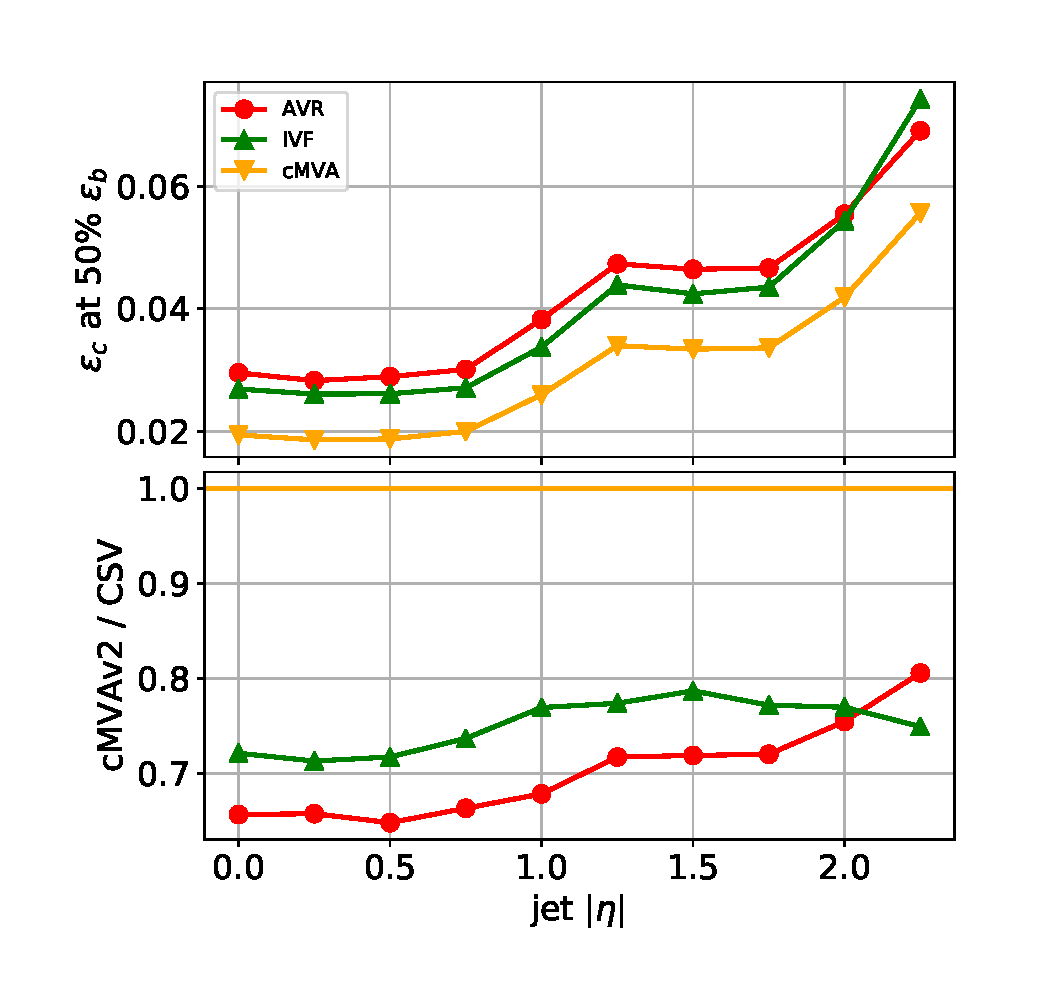
\includegraphics[width=0.5\textwidth]{figures/btv/tt_e50_c_eta.pdf}} \\
\caption[The cMVAv2 mistagging probability as a function of jet kinematics.]{The $p_T$ and $|\eta|$-dependent mistagging efficiency at a fixed $\epsilon_{b}$ in~\ttbar~+jets simulation. We compare the cMVAv2 discriminator to the CSV IVF and AVR discriminators in terms of the light jet and charm jet efficiency (mistagging) at the working point with~$50\%$~b~jet efficiency. We see that the cMVAv2 discriminator performs well over a wide~$p_T$~and~$|\eta|$~range, with $\epsilon_{\mathrm{light}}$ in the forward region being around~$40\%$ lower than for the CSV algorithm. While the efficiency of the algorithm overall still depends on jet kinematics due to the inherent correlation between the kinematics and the underlying variables sensitive to b-tagging, the dependence is somewhat lower for cMVAv2 than for CSV.}
\label{fig:btag_kinematics}
\end{centering}
\end{figure}

The final validation and calibration of the cMVAv2 algorithm was done using the tag counting method, where the b~tagging efficiency and the corresponding scale factor between data and simulation is determined from \ttbar+jets dilepton events relying on the $\mathrm{t} \rightarrow \mathrm{b} \mathrm{W}^+$ decay and thus the presence of 2 true b~jets. The correction for the light jet mistagging efficiency is extracted from multi-jet events based on the discriminator distribution using jets with only negative impact parameters and thus enriched in light jets. The cMVAv2 discriminator corrections have independently been determined with the differential reweighting method described further in~\cref{sec:object_id_btag} and the results are compatible with scale factor derived from tag counting~\cite{CMS-PAS-BTV-15-001}. 

The evaluation of the cMVAv2 b~tagger has been implemented in \texttt{CMSSW} independently of the optimisation. As such, the cMVAv2 was one of the two default b discriminators of CMS during the 2016 data-taking period. In order to interface the decision trees optimised using \texttt{scikit-learn} to the CMS online software in \texttt{CMSSW}, we have developed a stand-alone library~\cite{mlglue} to convert between BDT implementations form several commonly used open source machine learning toolkits, namely \texttt{scikit-learn}, \texttt{xgboost} and \texttt{TMVA}. The set of decision trees was then exported as a stand-alone payload to the~\texttt{CMSSW} environment, such that the cMVAv2 b~discriminator could be deployed through standard reconstruction software by simply evaluating the decision trees.

\section{Summary}
We have developed an improved b~tagging algorithm, the cMVAv2, for Run II which combines the discrimination power in several independently optimised b~discriminators using different vertexing algorithms and different subsystems of the detector. The cMVAv2 b~discriminator outperforms the present state of the art at CMS by  
The cMVAv2 algorithm was optimised using BDT algorithsm commonly used in the  